\chapter{防火墙和网络地址转换}

\section{引言}

在因特网(Internet)以及协议发展的最初几年,大多数网络设计师和开发人员都来自于
大学或其他从事研究的机构。这些研究人员普遍是友好和合作的,当时的互联网系统虽然容
易遭受攻击,但并没有多少人有兴趣去攻击它。在20世纪80年代末,特别是20世纪90年
代初至中期,互联网得到了大家的普遍关注,致使人们开始感兴趣去攻陷它。成功的攻击成
了家常便饭,互联网主机在软件实现中的各种错误及未定义的协议操作造成了大量问题。因
为一些网站有大量的、各种版本的操作系统软件,对于系统管理员而言,要确保所有这些后
端系统中的各种错误均已被修复是非常困难的。此外,对于已经被淘汰的系统,要完成这项
工作几乎是不可能的。为了解决这个问题,需要一种方法来控制互联网中网络流量的流向。
今天,这项工作由防火墙来完成,它是一种能够限制所转发的流量类型的路由器。

随着部署防火墙来保护企业,另一个问题变得越来越重要:可用的IPv4 地址数量正面
临枯竭的威胁。必须采取有效的措施来管理IP地址的分配和使用。除了IPv6之外,一种
最为重要的解决机制就是网络地址转换(Network Address Translation, NAT)。采用 NAT之
后,互联网地址就不再需要是全球唯一的,因此可以在互联网的不同部分(称地址范围
(address realm))被重复使用。允许在多个范围中的同一地址重复使用,大大缓解了地址耗
尽的问题。正如我们所看到的,NAT与防火墙相结合生成的复合设备,已经演变成用于连接
终端用户的最为常见的路由器类型,包括连接家庭网络和小型企业网络至互联网的。现在,
我们将进一步探讨防火墙和 NAT 的细节。

\section{防火墙}

保证终端系统的软件是最新的和不存在任何错误需要承担巨大的管理压力,因此确保终
端系统免受攻击的焦点转为如何利用防火墙来过滤部分流量以限制流量流向终端系统。今天
防火墙很常见,并已经演化出多种不同的类型。

最为常用的两种防火墙是代理防火墙(proxy firewall) 和包过滤防火墙(packet-filter
frewall)。它们之间的主要区别是所操作的协议栈的层次及由此决定的IP 地址和端口号的使
用。包过滤防火墙是一个互联网路由器,能够丢弃符合(或者不符合)特定条件的数据包。
从 Internet 客户端的角度来看,代理防火墙则是一个多宿主的服务器主机。也就是说,它是
TCP 和UDP 传输关联的终点,通常不会在IP 协议层中路由IP数据报。

\subsection{包过滤防火墙}

包过滤防火墙作为互联网路由器,能够过滤(filter)(丢弃)一些网络流量。它们一般
都可以配置丢弃或转发数据包头中符合(或不符合)特定标准的数据包,这些标准称为过
滤器(filter)。简单的过滤器包括网络层或传输层报头中各个部分的范围比较。最流行的过
滤器包括IP 地址或者选项、ICMP报文的类型,以及根据数据包中端口号确定的各种UDP
或TCP服务。正如我们将看到的,最简单的包过滤防火墙是无状态的,而更复杂的防火墙
是有状态的。无状态的包过滤防火墙单独处理每一个数据报,而有状态的防火墙能够通过
关联已经或者即将到达的数据包来推断流或者数据报的信息,即那些属于同一个传输关联
(transport association)的数据包或构成同一个 IP 数据报(参见第10章)的IP分片。IP 分片
使得防火墙的工作变得更复杂,无状态包过滤防火墙极易被其混淆。

图7-1所示为一个典型的包过滤防火墙。在这里防火墙是一个有着三个网络接口的互联
网路由器:一个“内”接口,一个“外”接口和第三个“非军事区”(DMZ)接口。DMZ子
网能够访问外联网或DMZ,其中部署的服务器可供互联网用户访问。网络管理员会安装过
滤器或访问控制列表(Access Control Lists,ACL)(ACL 列出了什么类型的数据包需要被丟
弃或转发的基本政策)到防火墙中。通常情况下,这些过滤器将会全力拦截来自外网的恶意
流量,但不会限制从内网到外网的流量。

图7-1 一个典型的包过滤防火墙的配置。防火墙作为IP 路由器位于一个“内”网和“外”网之间,
有时是在第三个“DMZ”或外联网,只允许某些特定的流量通过。一种常见的配置是允许所
有从内网到外网的流量通过,但相反的方向只允许小部分的流量。当使用一个 DMZ时,只允
许从 Internet 访问其中的某些特定服务

\subsection{代理防火墙}

包过滤的防火墙作为一个路由器可以选择性地丢弃数据包。其他类型的防火墙,如代理
防火墙,并不是真正意义上的互联网路由器。相反,它们本质上是运行一个或多个应用层网
关(Application-Layer Gateways,ALG)的主机,该主机拥有多个网络接口,能够在应用层
中继两个连接/关联之间的特定类型的流量。它们通常不像路由器那样做IP转发,虽然现在
已经有结合了各种功能的更复杂的代理防火墙。

图7-2说明了一个代理防火墙。对于这种类型的防火墙,防火墙内的客户端通常会做特
殊配置以便关联(或者连接)到代理防火墙,而不是连接到实际提供所需服务的真正的终端
主机。(能够和代理防火墙以这种方式交互的应用需要提供相应的配置选项。)通常这些防火
墙作为多宿主主机,即便具备IP转发的能力也是被禁用的。与包过滤防火墙一样,一种常
见的配置是为“外”接口分配一个全局路由的IP 地址,“内”接口分配一个私有的IP地
址。因此,代理防火墙支持使用私有地址范围。

图7-2 代理防火墙作为一个多宿主的 Internet 主机,终止在应用层的TCP 和UDP 的连接。它不像一
个传统的IP 路由器,而更像一个 ALG。单个应用程序或代理为了其所支持的每个服务,必须
具备和代理防火墙进行通信交互的能力

虽然这种类型的防火墙是非常安全的(一些人认,这种类型的防火墙从根本上比包过
滤防火墙安全),但它是以脆性(brittleness)和缺乏灵活性代价的。特别是,因这种类型
的防火墙必须为每个传输层服务设置一个代理,任何要使用的新服务必须安装一个相应的代
理,并通过该代理来操作发起连接。此外,必须配置每个客户端以便能够找到代理(例如,
使用Web 代理自动发现协议或WPAD[XIDAD],当然也有一些替代的方法,如所请的捕捉
代理就能够处理某种类型的所有流量,而不管其目标地址如何)。至于部署方面,这些防火
墙在所有被访问的网络服务均能提前确定的环境中能工作得很好,但是添加额外的服务可能
需要网络运营者的重大干预。

代理防火墙的两种最常见的形式是 HTTP 代理防火墙(HTTP proxy firewall) \href{https://www.rfc-editor.org/rfc/rfc2616}{[RFC2616]}
和 SOCKS防火墙(SOCKS firewall)\href{https://www.rfc-editor.org/rfc/rfc1928}{[RFC1928]}。第一种类型也称为 web 代理,只能用于
HTTP 和HTTPS 协议(Web),这些协议是非常普遍的,因此这些代理会被经常使用。这些
代理对于内网用户来说就像是 Web 服务器,对于被访问的外部网站来说就像是Web 客户
端。这种代理往往也提供 Web 缓存(Web cache)功能。这些缓存保存网页的副本,以便后
续访问可以直接从缓存中获取,而不再需要访问原始的web 服务器。这样做的好处是可以
减少显示网页的延迟,提高用户访问网站的体验。一些Web 代理也经常被用作内容过滤器
(content filter),能够基于“黑名单”来阻止用户访问某些Web 网站。相反,在互联网上还
可以找到一些所谓的隧道代理服务器(tunneling proxy server)。这些服务器(例如 psiphon 和
CGIProxy)本质上执行相反的功能,以避免用户被内容过滤器封阻。

SOCKS协议比 HTTP 代理访问使用更为广泛,可用于 Web 之外的其他服务。目前正在
使用的SOCKS有两个版本:版本4和版本5。第4版为代理传输提供了基本的支持,而第
5版增加了强大的认证、UDP 传输和 IPv6 寻址。为使用SOCKS代理,应用程序在开发时必
须添加SOCKS 代理支持功能(即它必须是能够被代理的),同时通过配置应用程序能够获知
代理的位置及其版本。一旦配置完成,客户端使用SOCKS协议请求代理进行网络连接,也
可以选择性地进行 DNS查找。

\section{网络地址转换}

NAT本质上是一种允许在互联网的不同地方重复使用相同的IP地址集的机制。建立
NAT的主要动机是正在急剧减少的有限IP地址空间。使用 NAT最常见的情况是,唯一与
Internet 连接的站点仅被分配了很少的几个 IP 地址(甚至只有一个IP地址),但是内部却有
多台主机需要同时上网。当所有进出的流量均通过一个单独的NAT设备时,该设备将内部
系统的地址空间和全球互联网地址空间分割开,因此所有的内部系统可以使用本地分配的私
有IP 地址访问互联网。然而,为分配了私有地址空间的系统在互联网上提供服务是一项更
为复杂的工作。我们在7.3.4 节讨论这种情况。

NAT 的引入用以解决两个问题:IP地址枯竭和关于路由可扩展性的担忧。在刚推出的
时候(20世纪90年代初),NAT 仅作为权宜之计,是一种临时的措施,直到一些具有更大地
址数量的协议(最终是IPv6)被广泛部署止。无类域间路由(CIDR,见第2章)的发展解
决了路由可扩展性问题。NAT 是受欢迎的,因为它减少了对具备全局路由的互联网地址的需
求,同时提供了一些防火墙功能,并且仅需要很少的配置。但具有讽刺意味的是,快速发展
和广泛使用的 NAT 却严重影响了IPv6的推进进程。在IPv6 的诸多益处中,其中一项就是使
得不再需要 NAT\href{https://www.rfc-editor.org/rfc/rfc4864}{[RFC4864]}。

NAT 尽管很流行,但是存在几个缺点。最明显的是,需要做特殊配置才能使处于 NAT
内部的主机能够提供可供互联网访问的服务,因为互联网上的用户无法直接访问具备私有地
址的主机。此外,为了使NAT正常工作,每一个隶属于同一个连接或关联的双向数据包都
必须通过相同的NAT。这是因为NAT必须重写每个数据包的寻址信息,以便私有地址空间
的系统和 Internet 主机之间能够正常通信。在许多方面,NAT和互联网协议的基本宗旨是背
道而驰的:“智能边缘”(smart edge)和“哑巴中间”(dumb middle)。为完成工作,NAT 需要
跟踪每个关联(per-association)(或每个连接(per-connection))的连接状态,其操作贯穿多
个协议层,并不像传统的路由器。修改IP 层地址也需要同时修改传输层的校验码(见第10
章和第13 章关于伪头部的校验)。

NAT会对一些应用协议造成困扰,尤其是那些在应用层的有效载荷内记录IP地址信息
的协议。文件传输协议(File Transfer Protocol, FTP)\href{https://www.rfc-editor.org/rfc/rfc0959}{[RFC0959]}和 SIP\href{https://www.rfc-editor.org/rfc/rfc5411}{[RFC5411]}就是这种
类型的协议代表。它们需要一种特殊的应用层网关功能来重写应用程序的内容,以便能够毫
无修改地采用NAT或者其他的 NAT传输方法工作,这些传输方法允许应用程序自行确定如
何在NAT上工作。关于NAT的一个更完整的问题清单出现在\href{https://www.rfc-editor.org/rfc/rfc3027}{[RFC3027]}。尽管存在许多问
题,但 NAT 的使用非常广泛,并且被大多数网络路由器(基本上包括所有低端家用路由器)
所支持。今天,NAT是如此普遍,以至于应用程序设计者被鼓励开发“NAT友好”的应用
\href{https://www.rfc-editor.org/rfc/rfc3235}{[RFC3235]}。值得一提的是,尽管存在缺点,但是 NAT 所支持的基本协议(例如,电子邮件
和浏览器)被数以百万计的客户端系统在访问互联网时所采用。

NAT的工作原理就是重写通过路由器的数据包的识别信息。这种情况常发生在数据传输
的两个方向上。在这种最基本的形式中,NAT需要重写往一个方向传输的数据包的源IP地
址,重写往另一个方向传输的数据包的目的IP 地址。这允许传出的数据包的源IP 地址变为
NAT 路由器中面向 Internet 的网络接口地址,而不是原始主机的接口地址。因此,在互联网
上的主机看来,数据包是来自于具备全局路由IP 的 NAT路由器,而不是位于 NAT 内部的私
有地址的主机。

大多数的 NAT 同时执行转换(translation)和包过滤(packet fltering),包过滤的标准取
决于 NAT的动态状态。包过滤策略的选择可能会有不同的粒度,例如,NAT如何处理非请
求的数据包(它们和源自于 NAT 内部的数据包没有任何关联)取决于源和目标IP 地址和/或
源和目的端口号。处理的行为在不同的NAT上会有所不同,有时甚至在同一个 NAT上也会
随时间变化而变化。这为必须运行在 NAT后面的应用程序带来了各种挑战。

图7-3 一个将私有地址及其内部系统与互联网隔离的 NAT。私有地址的数据包不会在互联网上直接
路由,相反在进入和离开私有网络时必须通过 NAT 路由器。互联网主机看到流量来自于 NAT
的一个公共 IP 地址

\subsection{传统的 NAT:基本 NAT 和 NAPT}

很多年来都没有精确定义NAT的行为。尽管如此,根据 NAT思想行为的不同实现,已
经对出现的 NAT类型进行了分类。所谓的传统 NAT (traditional NAT)包括基本 NAT (basic
NAT)和网络地址端口转换(Network Address Port Translation,NAPT) \href{https://www.rfc-editor.org/rfc/rfc3022}{[RFC3022]}。基本
NAT 只执行IP 地址的重写。本质上就是将私有地址改写一个公共地址——往往取自于一
个由ISP提供的地址池或公有地址范围。这种类型的NAT 不是最流行的,因为它无助于减
少需要使用的IP 地址数量,全局可路由的地址数量必须大于或等于希望同时访问 Internet 的
内部主机数量。一个比较流行的做法是采用 NAPT。NAPT使用传输层标识符(即TCP和
UDP 端口,ICMP 查询标识符)来确定一个特定的数据包到底和NAT 内部的哪台私有主机关
联(见图7-4)。这使得大量的内部主机(即好几千台)能够同时访问互联网,而使用的公有
地址数量却很少,通常只需要一个。除非进行区分很重要,否则我们所说的 NAT将同时包
括传统的 NAT 和 NAPT。

图 7-4
一个基本的IPv4 NAT(左)利用地址池中的地址重写IP 地址,但是保留端口号不变。NAPT(右)
也称为IP 伪装,通常将所有的地址都重写到一个地址。NAPT 有时必须重写端口号,以避免冲
突。在这种情况下,第二个实例的端口号23479被重写为3000,以便区分返回的192.168.1.2 和
192.168.1.35 的流量

在NAT“后面”或者“内部”使用的私有地址范围不受除了本地网络管理人员之外的任
何人的限制。因此,有可能在私有范围内采用全局地址空间。原则上,这是可以接受的。然
而,当这样的全局地址也被互联网上的另一个实体所使用时,在私有范围内的本地系统极有
可能无法达到使用相同地址的公共系统,这是因为采用相同地址的本地系统会屏蔽掉使用相
同地址的远端系统。为了避免这种不良情况的发生,保留了三个 IPv4地址范围作为私有地
址范围使用[RFC1918中]:10.0.0.0/8,172.16.0.0/12,192.168.0.0/16。这些地址范围经常
被用来作为嵌人式 DHCP 服务器(见第6章)的地址池的默认值。

正如刚才所说,NAT 提供了一定程度上的类似于防火墙的安全性。默认情况下,从互联
网上无法访问 NAT私有端的所有系统。在大多数NAT 部署中,内部系统使用私有地址。因
此,必须借助NAT 的参与(根据其使用策略和行),才能保证私人地址领域和公共领域中
的主机之间的正常通信。虽然在实践中可以使用各种策略,一个共同的策略是:几乎允许所
有的传出及其返回流量(与传出流量相对应的)通过NAT,但几乎阻断所有传入的新连接请
求。此行为抑制了试图确定可利用的活动主机的IP地址“探测”攻击。此外,NAT(尤其是
NAPT)对外“隐藏”内部地址的数量和配置。一些用户认为这些拓扑信息是专有的,并应
保密。NAT 有助于这种所谓的拓扑隐藏。

正如我们所探讨的,NAT需要适合它们所支持的协议和应用程序,所以很难在隔离
NAT所处理的协议的条件下单独讨论 NAT的行为。因此,我们现在考察NAT是如何处理其
支持的每个主要传输协议的,以及如何在IPv4/IPv6 混合环境中被使用。这其中的许多行力
细节一直是 IETF 的 BEHAVE(Behavior Engineering for Hindrance Avoidance) 工作组的讨论
主题。从2007年开始,BEHAVE 已经完成了一些文件,阐明了 NAT的一致行为。这些文件
对于应用程序编写者和 NAT 开发者是非常有用的,可以了解 NAT 是如何操作的。

\subsubsection{NAT 和 TCP}

回想第1章介绍的内容,互联网中最为主要的传输层协议是TCP,使用一个IP地址和
端口号来标识一个连接的每一端。每个连接由两端组成,每个TCP连接由两个IP地址和
两个端口号唯一标识。当发起一个 TCP连接时,“主动发起者”或客户端通常发送同步包
(SYN)到“被动发起者”或服务器端。服务器端通过回复一个自己的SYN 数据包进行响应,
同时还包括一个对客户端的SYN数据包进行确认的ACK数据包。客户端回复一个 ACK数
据包给服务器端。这样,通过“三次握手”创建了连接。类似的结束(FIN)数据包被用于优
雅地关闭连接。当然,连接也能通过重置(RST)数据包来强行关闭(请参阅第13章TCP连
接的详细描述)。与TCP 相关的传统 NAT 行为要求定义在\href{https://www.rfc-editor.org/rfc/rfc5382}{[RFC5382]}中,主要涉及了 TCP
的三次握手。

以图7-3中的家庭网络为例,考察一个由地址为10.0.0.126的无线客户端发起的TCP 连
接,其目标是 Web 服务器主机www.isoc.org(IPv4地址212.110.167.157)。使用以下符号
来表示 IPv4 地址和端口号:(源IP:源端口;目标IP:目标端口),在私人段内发起连接的
数据包可表示为(10.0.0.126:9200;212.110.167.157:80)。NAT/防火墙设备作为客户端的默
认路由器,将会收到第一个数据包。NAT注意到传人的数据包是一个新的连接(因TCP
报头中的SYN标志位是打开的,见第13章)。如果策略允许(通常会,因为这是一个向外
发起的连接),数据包的源IP 地址会被修改为 NAT 路由器的外部接口的IP地址。因此,当
NAT 转发这个数据包的时候,其寻址是(63.204.134.177:9200;212.110.167.157:80)。除了
转发数据包之外,NAT还创建一个内部状态记住当前正在处理一个新连接(称NAT 会
话(NAT session))。这种状态至少包括一个由客户端的源端口号和IP地址组成的条目(称
为NAT 映射(NAT mapping))。当 Internet 服务器回复时会用到这些信息。服务器会采用客
户端初始选择使用的端口号来回复端点(63.204.134.177:9200),即 NAT的外部地址。这种
行为被称为端口保留(port preservation)。通过比对收到的数据包的目的端口号与NAT映
射条目,NAT能够确定发起请求的客户端的内部IP地址。在我们的例子中,这个地址是
10.0.0.126,所以NAT将回复的数据包从(212.110.167.157:80;63.204.134.177:9200)改
(212.110.167.157:80;10.0.0.126:9200),并对其进行转发。然后客户端收到对其请求的响应,
这样在多数情况下表示已经连接到服务器。

这个例子说明了在正常情况下是如何建立一个基本NAT会话的,但并未说明该会话是
如何被清除的。会话状态将会在交换 FIN数据包之后被删除,但并不是所有的TCP连接都
是正常关闭的。有时只是简单地将主机关闭,这样会导致应该被清除的NAT 映射仍保留在
内存中。因此当流量很少时(或者用一个 RST段表示存在其他问题),NAT 必须清除这些被
认为已经“死亡”的映射条目。

大多数的 NAT包括一个TCP连接建立的简化版本,并可以区分连接成功还是失败了。
特别地,NAT 在检测到一个传出的 SYN数据包后会激活连接计时器(connection timer),如
果回复的ACK数据包在计时器到期之前还未到达,则该会话状态将被清除。如果 ACK 数据
包到达了,计时器将被清除,并创建一个超时较长的会话计时器(session timer)(如用小时来
代替分钟)。当发生这种情况时,NAT 可能会向内部的端点发送一个额外的数据包,用于确
认该会话是否已经终止了(称为探测(probing))。如果收到ACK,NAT认识到该连接仍然
是活跃的,则重置会话计时器,并不会删除会话。如果没有收到响应(在关闭计时器(close
timer)超时之后)或者收到一个 RST数据包,表明该连接已经终止,状态将被清除。

\href{https://www.rfc-editor.org/rfc/rfc5382}{[RFC5382]}是BEHAVE 工作组的一个成果,指出一个 TCP 连接可以被配置发送“存
活”(keepalive) 数据包(见第17章),在该配置被启用时其默认的发送速率是每两个小时一
个数据包。否则,一个TCP 连接可以一直保持下去。然而,当一个连接被建立或清除时,
其最大的空闲时间是4分钟。因此,\href{https://www.rfc-editor.org/rfc/rfc5382}{[RFC5382]}要求(REQ-5)NAT 在判定所创建的连接是
否已经断开前至少需要等待2小时4分钟,而在判定部分打开或关闭的连接是否已经断开前
至少需要等待4分钟。

一个TCP NAT 面临的棘手问题是如何处理位于多个NAT 内部的主机上运行的对等
(peer-to-peer)应用\href{https://www.rfc-editor.org/rfc/rfc5128}{[RFC5128]}。一部分应用程序采用了“同时发起连接” (simultaneous open)
的技术,让连接的每一端均作为客户端同时发送 SYN数据包。TCP能够响应 SYN+ACK 的
数据包,完成连接的速度比三次握手还要快,但目前有许多 NAT并不能正确地处理这种情
况。为此,\href{https://www.rfc-editor.org/rfc/rfc5382}{[RFC5382]}要求(REQ-2)NAT处理所有有效的TCP包交换,尤其是这种连接同
时打开的情况。某些对等应用程序(如网络游戏)便采用了这种行为。此外,\href{https://www.rfc-editor.org/rfc/rfc5382}{[RFC5382]} 还
规定 NAT 将会静默丢弃那些一无所知的传人的SYN数据包。这可能会发生在同时发起一个
连接时,即当外部主机的SYN 数据包先于内部主机的SYN数据包到达 NAT 主机时。虽然这
种情况发生的可能性不大,但在出现时钟错误时确实会发生。如果传入的外部SYN数据包被
丢弃,内部的SYN 数据包还有时间来建立这个由外部的SYN数据包代表的NAT 映射。如果
在6s之内没有接收到内部的SYN数据包,NAT 可能会向外部主机发送一个错误信号。

\subsubsection{NAT 和 UDP}

针对单播 UDP的NAT 行要求定义在\href{https://www.rfc-editor.org/rfc/rfc4787}{[RFC4787]}中。NAT 在处理一系列 UDP 数据报
时所出现的问题,与处理TCP 时出现的问题大多数一样。但是UDP 有些不同,不像TCP,
它没有连接建立和清除的过程。更具体地说,它没有标识位,如用SYN、FIN 和 RST这些
位来表示一个会话的创建或销毁。此外,一个关联中的参与者也未必完全清楚。UDP 不像
TCP那样采用一个4元组来标识一个连接,相反,它是基于两个端点的地址/端口号的组
合。为了处理这些问题,如果一个绑定在“近期”没有被使用,UDP NAT会采用一个映射
计时器(mapping timer) 来清除 NAT的状态。用多大的计时器值来表示“最近”变化很大,
而\href{https://www.rfc-editor.org/rfc/rfc4787}{[RFC4787]}要求计时器至少2分钟,推荐5分钟。一个相关的问题是计时器何时刷新。
当数据包从内部传输到外部时 NAT就刷新(NAT 的对外刷新行为)或反之亦然(NAT 的对
内刷新行为)。\href{https://www.rfc-editor.org/rfc/rfc4787}{[RFC4787]}要求 NAT 保证对外的刷新行为。对内的刷新行为是可选的。

正如我们在第5章所讨论的(会在第10章再次看到),UDP 和IP 数据包可以被分片。
分片允许一个IP数据报跨越多个块(碎片),其中每个都是作为一个独立的数据报。但是,
由于UDP 是在IP 层之上,为此除了第一个分片之外,其他的分片并没有包含端口号信息,
而这是保证 NAPT正确操作所必需的信息。这同样也适用于TCP和ICMP。因此,在一般情
况下,分片并不能被NAT 或NAPT 正确处理。

\subsubsection{NAT 和其他的传输协议(DCCP,SCTP)}

尽管TCP 和UDP是迄今为止使用最广泛的互联网传输协议,但还有两种其他协议,
NAT已经为或正在为它们定义行为。数据报拥塞控制协定(Datagram Congestion Control
Protocol,DCCP)\href{https://www.rfc-editor.org/rfc/rfc4340}{[RFC4340]}提供拥塞控制的数据报服务。\href{https://www.rfc-editor.org/rfc/rfc5597}{[RFC5597]}给出了针对DCCP的
NAT 行为要求,\href{https://www.rfc-editor.org/rfc/rfc5596}{[RFC5596]}修改了DCCP 用于支持类似于TCP的同时发起连接的过程。流
控制传输协议(Stream Control Transmission Protocol,SCTP)\href{https://www.rfc-editor.org/rfc/rfc4960}{[RFC4960]} 提供了可靠的报文
处理服务,可容纳拥有多个地址的主机。[HBA09]及 [IDSNAT]给出了 NAT 与 SCTP 中应注
意的事项。

\subsubsection{NAT 和 ICMP}

ICMP 是Internet 控制报文协议,在第8章中有详细描述。它提供了关于IP数据包的状
态信息,也能够用于测量和收集网络状态信息。\href{https://www.rfc-editor.org/rfc/rfc5508}{[RFC5508]} 中定义了ICMP 的NAT 行为要
求。在ICMP 中使用NAT 时需要考虑两个问题。ICMP有两类报文:信息类的和出错类的。
出错类报文通常包含一个引起错误条件的IP 数据包(全部或部分)的副本。它们从错误被检
测到的端点,通常是在网络中,发送到数据报的原始发送方。按说,这并没有任何困难,但
是当一个ICMP错误报文通过 NAT 时,需要改写“错误数据报”的IP地址,以便它们能被
终端客户机识别(称为ICMP 的修复行动(ICMP fix-up))。信息类的报文也存在同样的问题,
但在这种情况下,大多数的报文类型是查询/响应或客户机/服务器性质的,还包括一个类
似于TCP 或UDP端口号的查询 ID (Query ID) 字段。因此,处理这些类型信息的 NAT 能够
识别向外传输的信息请求,并设置计时器用于等待响应。

\subsubsection{NAT 和隧道数据包}

在某些情况下,隧道数据包(见第3章)也需要通过NAT发送。当发生这种情况时,
NAT 不仅要修改IP 包头,还需要修改封装在其中的其他数据包的包头和有效载荷。一个这
样的例子是使用点对点隧道协议(PPTP,见第3章)的通用路由封装(GRE)包头。当GRE
包头通过NAT时,它的Call-ID 域会与NAT(或其他主机的隧道连接)冲突。如果 NAT没
能妥善处理这一映射,便不能通信。正如我们可以想象的,更多的封装层次只会使 NAT的
工作进一步复杂化。

\subsubsection{ NAT 和组播}

到目前为止,我们只讨论了 NAT的单播IP 流量。NAT 也可以被配置成支持组播流量
(见第9章),虽然这比较少见。\href{https://www.rfc-editor.org/rfc/rfc5135}{[RFC5135]} 给出了 NAT在处理组播流量时的要求。实际上,
为了支持组播流量,需要用IGMP代理来增强NAT(见\href{https://www.rfc-editor.org/rfc/rfc4605}{[RFC4605]}和第9章)。此外,从位
于NAT 内部的主机发送到外部的数据包的目的IP 地址和端口不会被修改。从内部传输到外
部的流量,其源地址和端口号可根据单播 UDP 行为修改。

\subsubsection{NAT 和 IPv6}

鉴于 NAT 在IPv4 中的广泛使用,很自然地会想到是否能够在 IPv6 中使用 NAT。目前,
这是一个有争议的问题\href{https://www.rfc-editor.org/rfc/rfc5902}{[RFC5902]}。对于许多协议设计者而言,NAT 出现了一个必要却不可
取的“缺点”—大大地增加了设计其他协议的复杂性。由于在IPv6 中没有必要节省地址
空间,而其他的NAT 特性(例如,防火墙功能,拓扑隐藏和隐私)也能通过本地网络保护
(Local Network Protection, LNP)来提供,因此人们坚决抵制在 IPv6 中使用 NAT \href{https://www.rfc-editor.org/rfc/rfc4864}{[RFC4864]}。
LNP 代表在 IPv6 中达到或者超过 NAT 性能的技术集合。

除了具备包过滤属性,NAT还支持多个地址范围共存,能够避免当站点切换ISP 时需
要改变其IP 地址的问题。例如,\href{https://www.rfc-editor.org/rfc/rfc4193}{[RFC4193]}定义了唯一的本地 IPv6 单播地址(Unique Local
IPv6 Unicast Addresses,ULA),能够为被称 NPTv6\href{https://www.rfc-editor.org/rfc/rfc6296}{[RFC6296]}的尚处于实验阶段的IPv6
到IPv6前缀转换所来用。它采用了一种算法而不是一个表格,基于前缀将一个 IPv6 地址转
换其他的(不同的)IPv6地址(例如,在不同的地址范围中),因此不需要像传统的NAT
那样需要维护单个连接的状态。此外,该算法需要修改地址以保证通用传输协议(TCP,
UDP)的“校验和”计算值保持不变。由于不需要修改网络层之上的数据包中的数据,也不
需要访问传输层的端口号,因此该方法显著地降低了 NAT的复杂性。然而,需要访问 NAT
外部地址的应用程序必须使用NAT 穿越方法或依赖于 ALG。此外,NPTv6 本身并不提供防
火墙的包过滤功能,因此必须考虑额外的部署。

\subsection{地址和端口转换行为}

NAT 的操作方式差别很大。大部分的细节涉及具体的地址和端口映射。IETF 工作组
BEHAVE 的主要目标之一是要阐明共同行为,规定哪些是最合适的。为了更好地理解所涉及
的问题,我们从一个通用的 NAT 映射例子开始(见图7-5)。

在图7-5中,我们使用符号X:表示在私有地址范围(内部主机)中的主机使用IP地址
X、端口号x(对于ICMP,采用查询ID 代替端口号)。通常 X取自于定义在\href{https://www.rfc-editor.org/rfc/rfc1918}{[RFC1918]}中的
私有IPv4地址空间。为了连接到远程地址/端口组合Y:y,NAT 需要使用一个外部地址(通
常是公共的和全局路由的)X1'和端口号x1'来创建一个映射。假设内部主机先连接到 Y1:Y1,
再连接到 Y2:y2,NAT则需先创建映射X1':x1’,再创建映射X2’:x2’。在大多数情况下,X1'
等于X2’,因为大多数网站只使用一个全局路由的IP地址。如果x1’等于x2’,映射则被认为
是重复使用的。如果x1’和x2’均与*相等,NAT 实现前面提到过的端口保留。在某些情况
下,端口保留是不可能的,所以 NAT必须处理图7-4所示的端口冲突。

图7-5 NAT地址和端口行为是由映射基于的内容刻画的。内部主机使用IP地址:端口X:x来联系
Y:y/ 和 Y2:y2。在NAT这些关联中使用的地址和端口分别是X1':x1’和X2‘:×2’。如果对于任何
Y1:y1 或者Y2:32,X1':x!'等于X2‘:x2’,则NAT 存在独立于端点的映射。若当且仅当Y1等于
12时,X1'’ I'才等于X2’:×2’,则NAT存在地址相关的映射。若当且仅当 Y1:p1 等于Y2:22时,
X1':x1'才等于X2':x2’,则NAT存在地址和端口相关的映射。若NAT的外部地址是在没有考
虑内部或者外部地址情况下选择的,则拥有多个外部地址的NAT(即其中X1'可能不等于 X2'
有一个任意地址池行为。另外还有一个选择,它可能有一个配对池行为,在这种情况下任何与
Y1 相关的关联均使用相同的X1

表7-1 和图7-5概括了由\href{https://www.rfc-editor.org/rfc/rfc4787}{[RFC4787]}定义的各种 NAT端口和地址行为。表7-1使用类
似的术语定义了在7.3.3节中介绍过的过滤行为。在所有常见的传输层协议中,包括TCP 和
UDP,所需的NAT地址和端口处理行为是独立于端点的(在ICMP中推荐使用类似行为)。
这项规定的目的是帮助应用程序确定一个确保流量能够正常工作的外部地址。我们将在7.4
节讨论 NAT穿越时加详细地讨论这些。

\iffalse
\begin{table}[htbp]
	\centering
	\caption{ NAT 的全局行为将由其转换和过滤行为定义。这些都可能是独立于主机地址、依赖于地址,或依赖于地址和端口号}
	\begin{tabularx}{\textwidth}{bss}
		% \hline
		行为名称 & 转换行沩 & 过滤行为 \\ \hline
		独立于端点的 & 对于所有的 Y2:y2,X1':x1'=X2':x2'(必需的) & 只要任何X1':x!’存在,就允许X1:x1 的任何数据包(推荐用于最大透明性) \\
		依赖于地址的 & X1':x1'=X2':x2'当且仅当Y1 =Y2 & 只要X1之前联系过Y1,就允许从 Y1:y1 到X1:x1 的数据包(推荐用于更严格的过滤) \\
		依赖于地址和端口的 & X1':x1'=X2':x2’当且仅当Y1:y1 = Y2:Y2 & 只要X1之前联系过Y1:Vl,就允许从 Y1:1 到X1:x1 的数据包 \\ \hline
    \end{tabularx}
\end{table}
\fi

如前所述,NAT 可能有几个可用的外部地址。这个地址集通常被称 NAT池(NAT
pool) 或者 NAT地址池 (NAT address pool)。多数中型到大型的 NAT 使用地址池。请注意,
NAT地址池和在第6章中讨论的 DHCP地址池不同,当然一台设备可能需要同时处理 NAT
和DHCP地址池。在这种环境中的一个问题是,当位于 NAT后的一个主机同时发起多个连
接,此时是不是为每个连接分配相同的外部IP 地址(称为地址配对 (pairing)?如果没有
限制哪个外部地址用于关联,一个 NAT的IP 地址池的行为 (IP address pooling behavior)被
认为是任意(arbitrary)的。如果它实现地址配对,它就被称为被配对(paired)。配对是所有
传输层的推荐NAT行。如果未使用配对,内部主机的通信对等端可能会错误地断定,它
正与不同的主机进行通信。对于只有一个外部地址的 NAT,这显然不成问题。

一种脆弱的NAT 类型不仅需要重载地址,也需要重载端口(称端口重載(port
overloading))。在这种情况下,多个内部主机的流量可能被修改为相同的外部IP地址和端口
号(port number)。这是一种危险的情况,因为如果多台内部主机同时访问同一台外部主机
上的服务,那么当流量从外部主机返回时便无法找到适当的目的地址。对于TCP 而言,这
是由多个外部连接共享连接标识符的4元组(源和目标地址及端口号)所导致的结果。现在
这种行为是不允许的。

一些 NAT实现了一个特殊的功能,称为端口奇偶性(port parity)。这种 NAT 尝试保持
端口号(奇数或偶数)的奇偶性。因此,如果x1 是偶数,那么x1'也是偶数,反之亦然。虽
然不如端口保留那么强大,但这样的行为有时对于使用特殊端口的特定应用协议还是非常有
用的(例如,简称为RTP 的实时协议(Real-Time Protocol),历来使用多个端口,当然也有
方法来避免出现这种问题\href{https://www.rfc-editor.org/rfc/rfc5761}{[RFC5761]})。NAT 推荐保持端口的奇偶性,但并不是必需的。随
着更复杂的 NAT 传输方法的普及,这种特性也变得越来越不重要。

\subsection{过滤行}

当 NAT为一个TCP 连接、UDP 关联或各种形式的ICMP流量创建一个绑定,不仅要创
建地址和端口映射,作为一个防火墙,还必须确定返回流量的过滤行为,这是非常常见的情
况。NAT所执行的过滤类型,尽管在逻辑上与地址和端口处理行为不同,但常常是相关的。
尤其是使用相同的术语:独立于端点,依赖于地址,依赖于地址和端口。

一个NAT 的过滤行为通常与它是否已经建立了一个地址映射相关。显然,若NAT 中缺
乏任何形式的地址映射,那么它无法转发从外到内的任何流量,这是由于它不知道需要使用
的内部目标。对于外出流量最为常见的情况,是当创建一个绑定时,相关返回流量的过滤功
能将被禁止。对独立于端点的 NAT行为,只要为内部主机创建了映射,无论来源如何,都
将允许任何传入的流量。对依赖于地址的过滤行为,仅当X1:x1 之前访问过Y1 时,才允许
Y1:y1传输流量到X1:x1。对于那些依赖于地址和端口的NAT过滤行为,仅当X1:x1 之前访
问过Y:y1时,才允许 Y1:y1 传输流量到X1:x1。最后两个之间的区别是,后面那个只是将端
口号y1考虑进去了。

\subsection{位于 NAT 之后的服务器}

采用NAT的主要问题之一,就是从外网无法直接访问位于 NAT之后的主机提供的服
务。再次考虑图7-3中的例子。如果地址为10.0.0.3的主机向互联网提供服务,如果没有
NAT 的参与便无法被访问到,至少存在如下两个原因。首先,NAT作为互联网路由器,它
必须同意转发目的地为10.0.0.3的传入流量。其次,更为重要的是,从互联网无法路由到 IP
地址 10.0.0.3,互联网中的主机也无法识别该地址。相反,NAT的外部地址被用于查找服务
器,NAT必须妥善重写和转发到达服务器的适当流量,以便它可以操作。这个过程通常称为
端口转发 (port forwarding) 或端口映射(port mapping)。

通过端口转发,进入 NAT 的流量被转发到一个位于 NAT 后面的特定配置的目的地址。
通过采用 NAT端口转发,就可以让服务器给互联网提供服务,即使它们被分配了私有的、不
可路由的地址。端口转发,通常需要采用转发到的服务器的地址和端口号来静态配置NAT。
端口转发就像一个始终存在的静态 NAT映射。如果服务器的IP地址被更改,NAT必须更新
寻址信息。端口转发也有局限性,只有一个端口号集合用于绑定每个(IP 地址,传输协议)
组合。因此,如果 NAT 只有一个外部IP 地址,它量多将相同传输协议的一个端口转发到一
个内部机器(例如,它不能支持通过TCP 80端口访问内部的两台独立的Web 服务器)。

\subsection{发夹和 NAT 环回}

当客户希望访问位于同一个 NAT私有地址空间内的服务器时,会导致一个有趣的问题。
能够支持这种场景的 NAT 需要实现发夹(hairpinning) 或者 NAT 环回(NAT loopback)。参
考图7-6,假设主机X1试图建立一个到主机X2的连接。如果X1 知道私有地址信息,X2:×2,这
没有任何问题,因为可以直接进行连接。然而,在某些情况下X1 只知道公用地址信息,X2‘:×2’。
在这些情况下,X1借助NAT采用目的地址X2':x2'尝试连接X2。当NAT意识到在 X2':x2'和
X2:x2 之间存在映射,并将数据包转发到位于NAT私有地址空间内的X2:x2 时,会触发发夹过
程。此时会出现一个问题,目的是X2:x2的数据包头部中的源地址应该是X1:x1 还是X1':x1'?

如果 NAT给X2的发夹数据包的源地址信息是X1':x!',那么这种 NAT 被称为有“外部源 IP
地址和端口”的发夹行为。这种行为是 TCP NAT
所必需的\href{https://www.rfc-editor.org/rfc/rfc5382}{[RFC5382]}。之所以需要这种行,是为了均采用全局路由地址的应用能够识别对
方。在我们的例子中,X2可能期望一个来自于X1'(例如,因为第三方系统的协调)的连接。

图7-6 一个实现了发夹或者 NAT 环回的 NAT允许一个客户机使用服务器的外部IP
地址和端口号到达位于 NAT侧的服务器。也就是说,X1能够采用地址信息
X2':×2'到达 X2:x2

\subsection{NAT 编辑}

总之,大多数IP 流量均使用 UDP和TCP 传输协议在互联网上进行传输。这些传输协
议,自己就可以很好地被NAT 支持,而无须增加额外的复杂性,这是因为它们的格式是很
好理解的。当应用层协议与它们一起携带传输层或更低层的信息,如IP 地址,NAT的问题
就会变得复杂得多。最常见的例子是FTP\href{https://www.rfc-editor.org/rfc/rfc0959}{[RFC0959]}。在正常操作中,它交换传输及网络
层的端点信息(IP 地址和端口号),所以当要传输大量数据时可以增加额外的连接。这需要
NAT 不仅改写数据报的IP 和TCP部分中的IP地址和端口号,而且也需要修改有些应用的
有效载荷本身。具有这种能力的 NAT 有时也被称次 NAT编辑器(NAT editor)。如果 NAT改
变了包的应用载荷大小,接着需要更多的工作要做。例如,TCP 为数据传输中的每个字节分
配了一个序列号(见第15章),所以如果一个数据包的大小改变了,序列号也需要相应地修
改。PPTP\href{https://www.rfc-editor.org/rfc/rfc2637}{[RFC2637]}在进行透明操作时便需要 NAT编辑器(见第3章)。

\subsection{服务提供者 NAT 和服务提供者IPV6转换}

一个相对较新的发展方向是将 NAT 从客户端移动到ISP 端。这被称为服务提供者 NAT
(service provider NAT,SPNAT)、运营商级 NAT (carrier-grade NAT, CGN),或大规模 NAT
(large-scale NAT,LSN),目的是为了进一步减轻IPv4地址枯竭的问题。采用 SPNAT,可以
想象许多ISP 的客户可以共享一个单一的全局IPv4地址。实际上,这是将汇聚点从客户这
边转移到了ISP那边。在基本形式中,常规 NAT和 SPNAT 之间没有功能上的差昇,区别只
在于推荐的使用域。然而,将 NAT功能从客户端转移到 ISP端也带来了新的安全隐患,最
终用户是否能够部署网络服务器和控制防火墙策略也成了一个问题[MBCB08]。2009年以来
的研究发现,很多用户由于使用了对等程序,因此愿意接受进来的连接[ANM09]。

SPNAT 有助于解决IPv4地址枯竭的问题,但IPv6 才是最终的解决方案。然而出于各种
已经讨论过的原因,IPv6部署已落后于预期。最初,双协议栈方案(见\href{https://www.rfc-editor.org/rfc/rfc4213}{[RFC4213]}),即每
个系统同时使用IPv6和IPv4地址,被提出用于支持向 IPv6过渡,但这种做法在IPv4地址
耗尽之前只是暂时、不那么必要的。目前正在采用更为务实的方法,就是在各种配置中结合
隧道、地址转换、双协议栈系统多种技术。在介绍完为处理现有的 NAT 而开发的方法之后,
我们将在7.6节中探讨这些。

\section{NAT 穿越}

鉴于将ALG 和NAT编辑器放置于NAT 设备中的复杂性,一种可替代的方法是应用程
序自己尝试执行 NAT 穿越(NAT traversal)。此时应用程序需要确定其流量通过NAT 时使用
的外部IP 地址和端口号,并对其协议操作做相应的修改。如果一个应用程序分布在整个网络
中(例如,有多个客户端和服务器,其中一些并不在NAT后),服务器可为位于NAT 后的客
户端之间传递(拷贝)数据,或者使这样的客户端发现对方的NAT绑定,并促成它们之间的
直接通信。使用一台服务器在客户端之间进行数据拷贝是不得已的选择,因为这其中会涉及
负载和潜在的滥用。因此,大多数时候是尝试提供一些方法,以便允许客户机之间直接通信。
直接通信的方法在对等文件共享、游戏和通信应用中已经非常广泛。然而,这种技术

往往局限于某一特定的应用程序,这意味着每一个需要NAT 穿越的新分布式应用程序,均
倾向于实现自己的方法。这可能会导致冗余和互操作性问题,最终增加了用户的挫败感和成
本。为了应付这种情况,已经建立了一个处理NAT 穿越的标准方法,它取决于几个我们在
下面的章节中讨论的不同从属协议。现在,我们先从其中一个为分布式应用所采用、健壮但
尚未成为标准的方法开始。紧接着,我们来标准化 NAT 穿越的框架。

\subsection{针孔和打孔}

如前所述,一个 NAT通常包括流量重写和过滤功能。当一个 NAT映射创建时,针对特
定应用程序的流量通常允许在 NAT 的两个方向传输。这种映射是临时的,通常只适用于在
执行时间内的单一应用程序。这类映射被称针孔(pinhole),因为它们被设计为只允许通过
一部分的临时信息流量(例如,一对IP 地址和端口号组合)。随着程序之间的通信,针孔通
常动态地创建和删除。

通过采用针孔试图使位于 NAT之后的两个或两个以上的系统直接通信的方法称为打孔
(hole punching)。\href{https://www.rfc-editor.org/rfc/rfc5128}{[RFC5128]}的3.3节描述了针对UDP 的打孔,3.4节描述针对TCP 的打孔。
为了打一个孔,一个客户机需通过一个向外的连接来访问一台已知的服务器,这样便在本地
的NAT 中创建了一个映射。当另一个客户机访问同一台服务器时,由于服务器和每个客户
机均有连接,因此知道它们的外部寻址信息。它然后在客户机之间交换它们的外部寻址信
息。一旦知道了这个信息,一个客户机便可以尝试直接连接到其他的客户机。流行的对等应
用Skype 便使用了这种方法(和其他一些方法)。

参照图 7-7,假设客户机 A 访问服务器SI,然后客户机 B也访问服务器SI。S1 会知道
A 和B的外部寻址信息:分别为IPv4 地址192.0.2.201 和 203.0.113.100。将B 的信息发送给
A(反之亦然),A可以尝试利用B 的外部地址直接联系B(反之亦然)。这是否有效取决于已
部署的NAT类型。对于连接(A,S1),其NAT状态在 N1 中,对于连接(B,S1),其NAT状
态同时在N2 和N3中。如果所有 NAT独立于端点,这些信息便足够使直接通信成为可能。
由于任何其他类型的NAT将不会接受除了S1 之外的流量,从而阻止直接通信。换句话说,
如果两台主机均位于具备依赖于地址或者同时依赖于地址和端口映射行为的NAT之后,那
么这种方法是行不通的。

图7-7
位于 NAT后的客户机上运行的应用程序可能需要一台服务器的协助,以便能够直接进行通信。
在打孔中,专门运行特定应用程序的服务器客户机之间交换信息用以建立NAT状态,如果
可能的话便可直接进行通信。当通过 NAT 时,通过使用标准的通用协议,一些应用尝试“确
定”(确定和维护)其流量将被分配的地址(和端口号)。在某些情况下这些方法将会遇到麻烦,
如在多层次的NAT环境中。在这个例子中,在S1 中客户机 A的外部可见地址是192.0.2.201,
客户机B的是203.0.113.100。然而在S2 中,客户机B的外部地址是 10.0.1.1

\subsection{单边的自地址确定}

应用程序使用一系列方法来定位其流量在通过NAT 时所采用的地址。这便称为确定
(fxing)(学习和维护)地址信息。地址确定的方法分为直接和间接两种。间接方法涉及通过
与 NAT 交换流量来推测其行为。直接方法涉及应用程序和 NAT 本身之间通过一个或者多个
特殊协议(目前还不是IETF 的标准)来进行直接会话。IETF 花费了很大的精力来发展被特
定应用程序所广泛采用的间接方法,其中为最知名的便是VoIP 应用。目前部分 NAT 也能够
支持一些直接方法。这些方法也为 NAT的基本配置做准备,因此我们将在NAT 的安装和配
置中对其进行讨论。

在没有NAT协助的情况下一个应用程序尝试确定地址,所执行的地址确定被称为是
单边类型的。这样做的应用程序被称为是执行单边的自地址确定(UNilateral Self-Address
Fixing,UNSAF)「RFC34241。顾名思义,这种方法从长远来看被认为是不可取的,但暂时
却是必要的。UNSAF会涉及一套启发式,它们并不能保证在所有情况下都能工作,特别是
因为 NAT的行为受供应商和特定环境的影响变化很大。之前提到的BEHAVE文档,其目标
就是让NAT的行为更为一致。如果被广泛采用,UNSAF 方法工作起来将更为可靠。

在大多数感兴趣的情况下,UNSAF采用类似打孔的客户机/服务器操作方式,但增加
了普适性。图7-7说明了一些在这种情况下可能出现的危害。其中一个问题就是每一台 NAT
缺乏一个单一的“外部”地址范围。在这个例子中,在客户端B和服务器SI之间有两层
NAT。这种情况可能会导致复杂性。例如,如果B上的应用希望通过一台服务器的UNSAF
获得其“外”地址,根据它是和服务器S1 通信还是和服务器S2通信,将会收到不同的回复。
最后,因为 UNSAF使用不同于 NAT 的服务器,始终存在这种可能性,即 NAT的行为报告
会随时间而改变,或者与 UNSAF 方法报告不一致。

鉴于 NAT 和UNSAF存在的各种问题,IAB——一个在IETF 中被推选出来的架构顾问
组,指出 UNSAF 协议方案必须回答针对它们规格的考虑:

\begin{itemize}
    \item 定义一个“短期”的 UNSAF方案解决有限范围问题。
    \item 定义一个退出策略/过渡计划。
    \item 讨论什么设计方案使得该方法变得“脆弱”。
    \item 确定长期、完善的技术解决方案的要求。
    \item 讨论任何知名的实际问题,或已知的经验。
\end{itemize}

这是针对协议规范规定提出的一个不寻常的列表,但它来自于不同的 NAT 和NAT 穿越
技术之间长期存在的互操作性问题。尽管存在上述问题,UNSAF 方法还是被经常使用,部
分原因是当前许多 NAT并没有一致的行为。我们现在就来看看这些方法如何使用积木的方
式来构建强大的、通用的 NAT传输技术,以最大限度地促成位于 NAT后的系统之间的通
信,甚至使跨越多个 NAT 系统之间的通信成为可能,正如图7-7所示。

\subsection{NAT 的会话穿越工具}

一个UNSAF 和 NAT穿越的主要功能,就是NAT 会话穿越工具(Session Traversal
Utilities for NAT,STUN)\href{https://www.rfc-editor.org/rfc/rfc5389}{[RFC5389]}。STUN 源自于 UDP简单隧道穿越 NAT(Simple Tunneling
of UDP through NAT),现在被称“经典的STUN”。经典STUN已经在 VoIP/SIP 应用
中使用了一段时间,但已被修改为一个可以为其他需要NAT穿越的协议使用的工具。需
要完整 NAT 穿越解决方案的应用,建议先从我们将在7.4.5节讨论(例如,ICE 和 SIP出
站)的其他机制开始。这些框架可以以一种或多种特定方式来使用STUN,被称为STUN用
法(usage)。用法可能会扩展STUN 的基本操作、报文类型,或在\href{https://www.rfc-editor.org/rfc/rfc5389}{[RFC5389]}定义的错误代
码集。

STUN是一个相对简单的客户机/服务器协议,它能够在多种环境中确定在NAT 中使用
的外部IP 地址和端口号。它也可以通过保持激活的信息来维持当前的NAT绑定。它需要在
NAT 一侧存在一台有效的“其他”合作服务器,以及几台被配置了全局IP 地址的可在互联
网上被访问到的公共STUN服务器。STUN服务器的主要工作是回显发送给它的STUN 请求,
以确定客户端的寻址信息。与一般UNSAF方法相比,该方法并非万无一失。但是STUN的
好处是它并不需要修改网络路由器、应用协议或者服务器。它仅需要客户端实现STUN 请求
协议,以及至少一台在适当位置可用的STUN服务器。STUN被设想为一种“临时”的解决
方案,直到制定和实施更复杂的直接协议,或由于IPv6 的广泛采用而使得 NAT 成为过时的
(正如目前许多在创建之后被普遍使用了10年甚至更长时间的标准协议)。

STUN 操作使用UDP、TCP 或具备传输层安全性(Transport Layer Security,TLS)的
TCP(见第18章)。STUN 用法规范定义特定用法所支持的传输协议。它次UDP和TCP使
用3478端口,为TCP/TLS使用3479端口。STUN 基础协议有两种类型的事务:请求/ 响应
事务(request/response transactions)和标志事务(indication transactions)。标志不需要响应,
并可以通过客户机或服务器生成。所有的信息包含类型、长度、值次 0x2112A442 的魔术
cookie,以及一个随机的96 位事务ID 用于匹配请求与响应或调试。每个报文始于2个0位,
并可能包含零个或多个属性(attribute)。支持特定的 STUN使用的方法(method) 在 STUN
报文类型中定义。各种STUN参数,包括方法和属性数量,均由IANA[ISP]维护。属性有
自己的类型,并可以改变长度。在一个IP数据包中,基本的STUN头通常紧挨着 UDP 传输
头,如图7-8所示。

图 7-8
STUN报文总是以2个0比特位开始,并且封装在UDP 中,当然TCP也是允许的。报文类型
字段同时给出了方法(例如,绑定)和类型(请求,响应,错误,成功)。事务ID 是一个长为
96位的数字,用于匹配请求和响应,或者在标志情况中用于调试。每个 STUN报文能够包含0
个或者多个属性,这取决于 STUN 的特定用法

基本的STUN 头的长度是20字节(见图7-8),报文长度(Message Length)字段提供了
一个最大为216-1 字节的完整的STUN报文长度(报文长度字段不包括20字节的报头长度),
由于报文总是用多个4字节来填充的,所以长度字段的低2位总是为0。通过UDPAIP 发出
的STUN报文所形成IP 数据包,若预先知道路径MTU的大小,为避免分片,其大小应小于
MTU(见第10章)。如果不知道MTU,整个数据报的长度(包括IP 和UDP 头和任何选项)
应小于576个字节(IPv4)或1280字节(IPv6)。STUN没有规定如何处理回复的报文超过
相反方向路径 MTU 的情况,所以服务器应当安排使用大小适当的报文。

通过 UDP/IP 传递的STUN报文是不可靠的,因此STUN 应用程序都需要自己来实现可
靠性。这是通过重发认丢失的报文来实现的。重传间隔是通过估计向对方发送和接受一个
报文的时间来计算的,称为往返时间(round-trip time,RTT)。在我们讨论 TCP 时(见第14
章),RTT的计算及重传计时器的设置是一个需要重点考虑的地方。STUN使用了类似的做法,
但在标准的TCP 上稍做了修改。更多细节请参考\href{https://www.rfc-editor.org/rfc/rfc5389}{[RFC5389]}。通过 TCP/IP 或带有TLS/IP 的
TCP 来传输的STUN报文的可靠性问题由TCP来处理。基于TCP 的连接可以支持多个待定
的 STUN事务。

STUN的属性被编码在一个 TLV 布局中,这也为许多其他互联网协议所采用。TLV 的
类型和长度字段均是16比特,值部分是长度可变的(最多到64KB,如果支持的话),紧随其
后的是多个4字节的填充(填充的比特可能为任意值)。在同一个 STUN报文中,属性类型
可能会出现多次,尽管只有第一个对接受者来说才是必需的。属性值低于0x8000的是必须
包含(comprehension-required)的属性,而其他的则称为可选包含(comprehension-optional)
的属性。假如一个代理收到一个拥有必须包含属性的报文但却并不知道该如何处理,就生成
一个错误。到目前为止,多数定义的属性是必须包含的[ISP]。

\href{https://www.rfc-editor.org/rfc/rfc5389}{[RFC5389]}定义了一个称之为绑定(binding)的STUN 方法,能够在请求/响应或者标
志事务中用于地址确定和保持 NAT绑定。它同时定义了11个属性,如表7-2所示。
表7-2 定义在\href{https://www.rfc-editor.org/rfc/rfc5389}{[RFC5389]} 中的STUN,有时也称为STUN2,它取代了经典 STUN。
这11个属性可能被兼容于STUN2的客户机和服务器所使用

名称

值

目的/用途

包含一个地址簇指示器和反向传输层地址(IPv4或

MAPPED-ADDRESS

0x0001

USERNAME

0x0006

MESSAGE-INTEGRITY

0x0008

ERROR-CODE

0x0009

UNKNOWN-ATTRIBUTES

0x000A

REALM

0x0014

NONCE

0x0015

XOR-MAPPED-ADDRESS

SOFTWARE

0x0020

0x8022

ALTERNATE-SERVER

0x8023

FINGERPRINT

0x8028

IPv6)

用户名称和密码,用来检验报文的完整性(达到513

字节)

在STUN 报文中的报文证书代码值(参见第18章和

\href{https://www.rfc-editor.org/rfc/rfc5389}{[RFC5389]})

包括3位差错类型、8位差错代码值和长度可变的差

错文本描述

和差错报文一起使用来表示未知属性(每个属性16

位值)

指示长期信任的证书“范围”名称

为了阻止重放攻击,在请求和应答中选择性地携带的

非重复值

MAPPED-ADDRESS 的或(XOR)版本

发送报文的软件的文本描述(例如,制造商和版本号)

提供了另一个IP地址供客户机使用,与MAPPED-
ADDRESS一起被编码

报文的CRC-32 和 0x5354554E 进行异或(XOR),如
果使用的话必须是最后的属性(可选的)

参考图7-5,地址信息为X:x的客户机总是有兴趣确定X1':x1’,即反向传输地址
(reflexive transport address) 或者映射地址(mapped address)。位于 Y1:y1 的STUN服务器将
反向传输地址包含在一个STUN 报文的 MAPPED-ADDRESS 属性中,并将其回复给客户机。
MAPPED-ADDRESS 属性包含一个8位的地址族(Address Family) 字段,一个16位的端口
号(Port Number)学段,以及一个32位或128位的地址(Address)字段,这取决于地址族
字段(IPv40x01,IPv6为0x02)指定是IPv4还是IPv6。之所以包含这个属性是为了与
经典的STUN保持向后兼容。更重要的属性是 XOR-MAPPED-ADDRESS 属性,其中包含与
MAPPED-ADDRESS 完全相同的属性值,但需要与魔术 cookie 值(对于IPv4)或事务 ID与
魔术的cookie串联值(对于IPv6)异或。以这种方式使用异或值的原因是为了检测并绕过通
用ALG,防止它们查看和改写通过的任何IP地址。这种ALG 是很脆弱的,因为它们可能
改写像 STUN这样的协议所必需的信息。经验表明,在数据包负载中异或IP地址足以绕过
ALG。

一个 STUN 客户机,包括多数的VoIP 设备和软件电话应用如 pisua[PJSUA],初始时
均需要配置一个或者多个 STUN服务器的IP 地址或者名称。之所以希望使用 STUN服务
器是因为当该应用程序最终与对方对话时它能看到相同的IP 地址,尽管要确定可能有点困
难。通常使用布局在互联网中的STUN服务器(例如,stun.ekiga.net, stun.xten.com, numb.
viagenie.ca)便足够了。一些服务器能够通过DNS服务(SRV)记录来发现(参见第11章)。
图 7-9所示的就是一个 STUN 绑定请求的例子。

\begin{figure}[H]
    \centering
	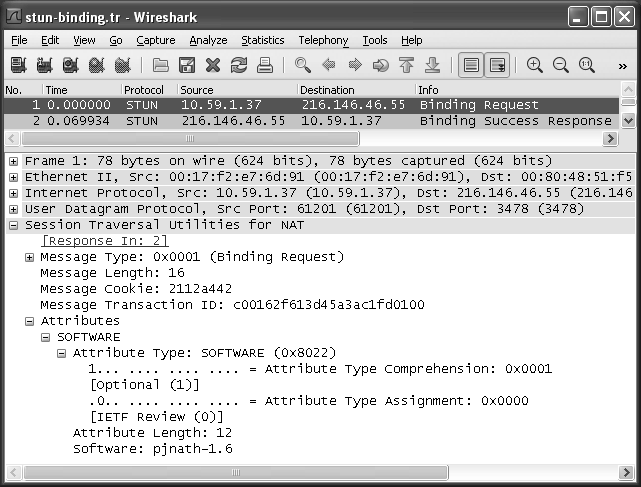
\includegraphics[scale=0.7]{imgs/7/7-9.png}
	\caption{一个 STUN绑定请求。该请求包含一个96位的事务ID 和一个用于识别发起请求的客户机的SOFTWARE 属性。属性包含了10个字符,但是其值向上舍人为4的倍数,给出的属性值是12。报文长度16 包含了用于包含属性类型和长度的4个字节(并未包含STUN头部)}
\end{figure}

图7-9所示的STUN 绑定请求例子由客户机先初始化。事务ID 是随机选择的,其请
求将被发送到 numb.viagenie.ca (IPv4 地址216.146.46.55 和216.146.46.59),这既是一台
STUN 服务器,也是一台 TURN服务器(参见7.4.4节)。请求中包含了用于识别客户应用的
SOFTWARE 属性。在这种情况下,请求由 pinath-1.6 初始化。这是包含在 pisua 中的 “PJSIP
NAT 助手”应用。信息长度包含用于属性类型和长度的4字节,加上用于保持属性的12个
字节。pjnath-1.6的长度只有10字节,但是属性长度总是向上取整为接近4字节的倍数。在
穿越过一个 NAT 之后,所得的应答如图7-10所示。

\begin{figure}[H]
    \centering
	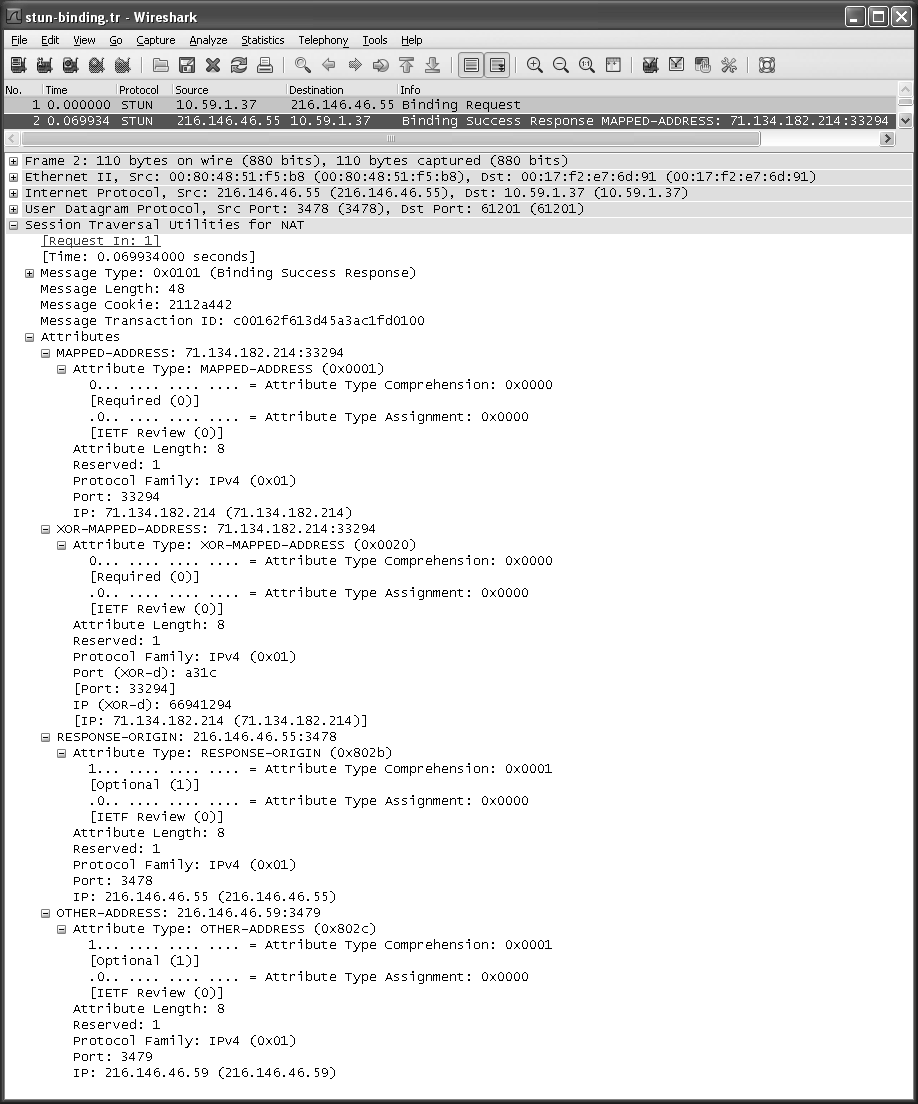
\includegraphics[scale=0.5]{imgs/7/7-10.png}
	\caption{包含4个属性的 STUN绑定回复。MAPPED-ADDRESS 和 XOR-MAPPED-ADDRESS 属性含服务器反向寻址信息。其他的属性用于实验性质的 NAT 行为发现机制\href{https://www.rfc-editor.org/rfc/rfc5780}{[RFC5780]}}
\end{figure}

图7-10所示的绑定回复以编码为属性集合的方式为客户机提供了有用的信息
MAPPED-ADDRESS 和 XOR-MAPPED-ADDRESS 属性表明,STUN服务器确定了服务
器反向地址71.134.182.214:33294。RESPONSE-ORGIN 和 OTHER-ADDRESS 属性被实系
设施用于发现NAT行为\href{https://www.rfc-editor.org/rfc/rfc5780}{[RFC5780]}。第一个属性给出了用来发送STUN报文的通信终端
(216.146.46.55:3478,与发送 IPv4地址和UDP端口号相匹配)。第二个属性表示假如客户村
请求“更改地址”或“改变端口”的行为,哪个IPv4源地址和端口号(216.146.45.59:3479
将被使用。后者的属性相当于现在已经过时的经典 STUN 中的 CHANGED-ADDRESS 属性。
如果一个请求要求变更地址或端口,如果可能,回复给客户机的协作 STUN服务器应该尝试
使用一个不同的地址。

STUN 可用于执行地址确定之外的其他一些称为机制(mechanisms) 的功能,包括 DNS
发现、重定向到备用服务器的方法和报文完整性交换。机制是在一个特定的STUN 用法的上
下文中选择的,所以一般被认是可选的STUN功能。一个更重要的机制是提供身份和报文
完整性验证。它有两种形式:短期信任机制(short-term credential mechanism) 和长期信任机
制(long-term credential mechanism)。

短期信任持续一个会话;特定时间由 STUN用法来定义。长期信任支持多个会话;它们
对应一个登录ID 或账户。短期信任通常用于特定的信息交换,长期信任在分配某些特定资
源时才使用(例如和TURN一起,见7.4.4节)。在能够被截获的地方,从来不用明文来发送
密码。

短期信任机制使用 USERNAME 和 MESSAGE-INTEGRITY这两个属性。两者在任何请
求中都是必需的。USERNAME 属性暗示需要哪种凭证,允许信息的发送方使用合适的共享
密码来形成一个报文的完整性校验(基于报文内容计算一个MAC值,见第18章)。使用短
期信任时,假定某种形式的凭证信息(例如,用户名和密码)在前期已经被交换过。用于形
成 STUN信息完整性校验的凭证被编码在 MESSAGE-INTEGRITY属性中。能够形成一个有
效的 MESSAGE-INTEGRIT属性值,意味着发送方当前持有的凭证是正确和最新的。

长期信任机制通过一种称为摘要挑战(digest challenge)的方法来保证凭证是最新的。
使用这个机制,客户端在初始化请求时不需要提供任何认证信息。服务器会先拒绝请求,但
在响应中会包含一个 REALM 属性。这可以被客户端用来确定需要提供何种凭证才能通过验
证,当然客户端可能有各种服务的凭据(例如,多个 VoIP 账户)。和 REALM一起,服务器
会提供一个永不重用的NONCE值,客户端能够用它来形成后续的请求。这种机制还采用了
MESSAGE-INTEGRITY属性,但其完整性功能是通过包含NONCE值来计算的。因此,偷
听了之前长期信任交换的窃贼很难回复一个有效的请求(因NONCE 值是不同的)。如何在
凭证中使用 NONCE及相关问题在第18 章有详细讨论。长期信任机制无法用来保护 STUN
标志,因为这些事务不是以请求/响应对来操作的。

\subsection{利用 NAT 中继的穿越}

利用 NAT 中继的穿越(Traversal Using Relays around NAT,TURN) \href{https://www.rfc-editor.org/rfc/rfc5766}{[RFC5766]}为两个
或多个系统提供了一种通信方式,即使它们均位于并未协作的NAT后。作为支持在这种情
况下通信的最后手段,它需要一个中继服务器在无法通信的系统之间传递数据。使用STUN
和一些 TURN特定报文的扩展,即使大多数其他方法都失败了它也能照样支持通信,只要每
个客户端均能连接到不在 NAT后的公共服务器。如果所有的NAT 均与 BEHAVE 标准兼容,
TURN 就没有必要存在了。直接通信的方法(即不使用TURN)总是优于采用TURN服务器
的方法。

根据图 7-11,通常位于 NAT后的TURN 客户机会访问位于公共互联网上的TURN服
务器,并暗示了它希望连接的其他系统(称对等(peer))。通过使用一种特殊的 DNS
NAPTR记录(见第11章和\href{https://www.rfc-editor.org/rfc/rfc5928}{[RFC5928]}),或通过手动配置,便可以找到用于通信的服务器的
地址和相应的协议。客户端从服务器端获得的地址和端口信息,称为中继传输地址(relayed
transport address),就是TURN 服务器用于和其他对等客户机通信的地址和端口号。客户端
也获得了它自己的服务器反向传输地址。对等客户机也得到了代表它们外部地址的服务器反
向传输地址。这些地址是客户端和服务器用来连接客户机及其对等所必需的。交换寻址信息
的方法并没有在TURN 中定义。相反,为了能够更加有效地使用TURN服务器,这些信息
必须使用其他一些机制来完成交换(例如,7.4.5节的ICE)。

图 7-11
根据\href{https://www.rfc-editor.org/rfc/rfc5766}{[RFC5766]},一个 TURN服务器通过中继来帮助位于“坏”(bad) NAT 之后的客户机之
间通信。客户端和服务器之间的流量可采用 TCP、UDP 或使用了TLS的TCP。服务器和一个
或多个对等客户机之间的流量使用UDP。中继是通信的最后手段,直接的方法才是首选

客户端使用 TURN 命令来创建和维护服务器上的分配(allocation)。一个分配类似于
一个多路NAT绑定,包括(唯一)中继传输地址,每个对等客户机需要使用它到达本机。
通过UDP/IPv4使用传统的TURN报文来发送服务器/对等数据。通过增强也能支持TCP
\href{https://www.rfc-editor.org/rfc/rfc6062}{[RFC6062]}和IPv6(IPv4和IPv6之间的中继)\href{https://www.rfc-editor.org/rfc/rfc6156}{[RFC6156]}。封装的客户/服务器数据内包括
发送信息或者接受相关数据的相应的对等客户机的信息。客户/服务器连接已被指定为使用
UDP/IPV4、TCP/IPv4 和来用TLS的TCPAIPv4。建立一个分配要求验证客户端的身份,通常
使用 STUN 长期信任机制。

TURN 支持两种客户端和对等之间拷贝数据的方法。第一种使用STUN方法来编码数
据,称为发送(Send)和数据(Data),定义在\href{https://www.rfc-editor.org/rfc/rfc5766}{[RFC5766]}中,这是 STUN 指示器 (indicator),
因此无须认证。其他的方法采用特定于 TURN 的概念,称为隧道(channel)。隧道是客户端
和对等之间的通信路径,相对于发送和数据方法负载较轻。通过隧道传递的报文使用一个较
小的、4个字节的报头,与TURN使用的较大的STUN格式报文是不兼容的。一个分配最多
可以拥有16K个隧道。发展隧道方法,有助于减小一些数据包比较小的应用的延迟和开销,
如VolP等。

在操作中,客户端使用一个 TURN定义的 STUN 分配(Allocate)方法来发出一个获取
分配的请求。如果成功,服务器响应一个成功指示器和已经分配的中继传输地址。如果客户
未能提供足够的验证信息,服务器可能会拒绝请求。现在,客户端必须发送更新的报文以保
持分配活跃。如果客户机10分钟内不发送信息,那么分配就到期,除非客户机在分配请求
中包含了一个用于指定不同生命周期值的 STUN LIFETIME 属性。通过请求一个生命周期
0的分配,就能将其删除。分配到期时,与其相关的所有隧道便也到期了。

分配通常使用“5元组”表示。在客户端,5元组包括客户端的主机地址和端口号、服
务器传输地址和端口号以及用于与服务器通信的传输协议。除了客户端的主机传输地址和端
口被替换服务器的反向地址和端口之外,服务器端使用了相同的五元组。一个分配可能有
零个或多个相关联的权限(permission),以限制允许通过TURN服务器的连接模式。每个权
限包括一个 IP 地址的限制,只有当源地址匹配的数据包到达TURN服务器,其数据有效载
荷才会被转发到相应的客户端。如果不能在5分钟内刷新,权限将被删除。

TURN通过6种方法、9个属性以及6个错误响应代码增强STUN。这些大致可以分为支
持建立和维护分配、认证以及操作隧道。6种方法和它们的方法号如下:分配(Allocate)(3),
刷新(Refresh)(4),发送(Send)(6),数据(Data)(7),创建权限(CreatePermission)(8),
隧道绑定(ChanneIBind)(9)。前两种方法用于建立并保持分配存活。Send和 Data 使用 STUN
报文封装从客户端发送到服务器的数据,反之亦然。GreatePermission 用于创建或刷新一个权
限,ChannelBind通过一个16位的隧道号与一个特定的对等客户端相关联。错误报文表明与
TURN 功能相关的问题,如认证失败或资源耗尽(例如,隧道数)。表7-3给出了由 TURN定
义的9个 STUN 属性名称、值以及目的。

表7-3

由 TURN 定义的 STUN属性

名称

CHANNEL-NUMBER

LIFETIME

XOR-PEER-ADDRESS

DATA

XO R-R ELAYED-ADDRESS

值

0x000C

Ox00OD

0x0012

0x0013

0x0016

EVEN-PORT

0x0018

REQUESTED-TRANSPORT

0x0019

DONT-FRAGMENT

0x001A

RESERVATION-TOKEN

0x0022

目的/用处

表示和数据关联的信道

请求分配超时(秒)

一个对等的地址和端口号,采用异或(XOR)编码

为一个发送或者数据指示保存数据

为一个客户机分配的服务器地址和端口

中继的传输层地址信息使用一个偶数端口的请求,
择性地按顺序请求分配下一个端口

一个客户机用来请求采用一个特定的传输层来形成传
输层地址,值来自于 IPv4 协议或者IPv6 下一跳头部字
段值

请求设置发送到对等数据包中的IPv4 头部中的“不分
片”位

服务器保存的一个中继传输层地址的唯一标志,这个
值作为一个引用提供给客户端

\begin{figure}[H]
    \centering
	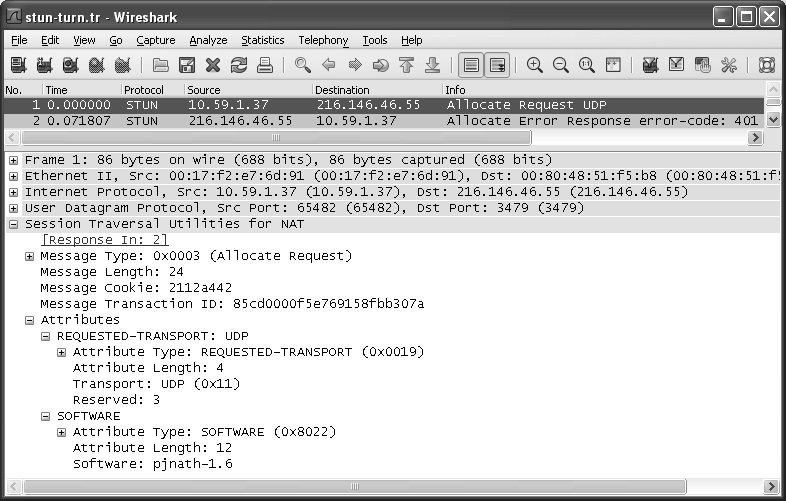
\includegraphics[scale=0.5]{imgs/7/7-12.png}
	\caption{TURN 分配请求是一个使用报文类型0x0003的STUN 报文。这一请求还包括 REQUE TRANSPORT 和SOFTWARE 属性。但是并未包含认证信息。根据STUN的长期信任,这个请求将失败}
\end{figure}

TURN 请求采用了STUN报文的形式,其中报文类型是一个分配请求。图7-12给出了
一个例子。根据STUN 的长期信任机制,图7-12所示的初始分配请求没有包括认证信息,
因此会被服务器拒绝。如图 7-13所示的一个分配错误响应表示服务器拒绝了请求。

\begin{figure}[H]
    \centering
	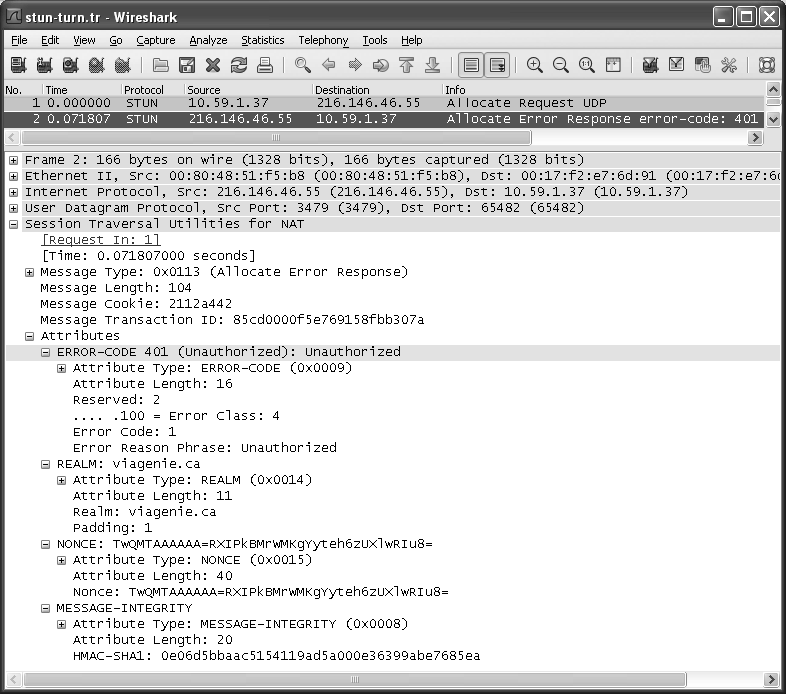
\includegraphics[scale=0.5]{imgs/7/7-13.png}
	\caption{TURN分配错误响应包含属性值为401的ERROR ̄CODE属性(未授权)。该报文是受完整性保护的,并包含了客户端为形成下一个认证分配请求所必需的REALM和NONCE属性}
\end{figure}

图7-13中的错误信息提供了 REALM属性(viagenie.ca)和客户端需要形成它下一个
请求的NONCE值。报文还包括了 MESSAGE-INTEGRITY 属性,所以客户端可以检查该
报文没有被修改,请求中属性 REALM 和 NONCE 是正确的。随后的请求中包含的属性有
USERNAME、NONCE 和 MESSAGE-INTEGRITY。参见图 7-14;

\begin{figure}[H]
    \centering
	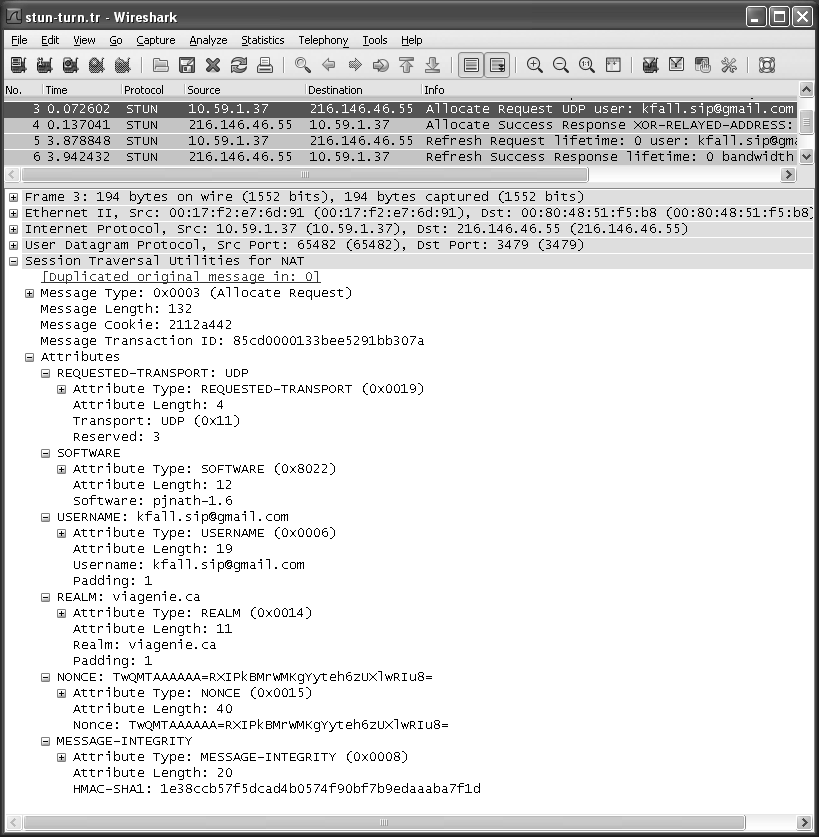
\includegraphics[scale=0.5]{imgs/7/7-14.png}
	\caption{第二个 TURN 分配请求包括了 USERNAME、REALM、NONCE 和 MESSAGE-INTEGRITY 属性。使用这些服务器能够验证报文的完整性及客户端的身份。如果成功,服务器将验证请求并分配}
\end{figure}

如图7-14所示,在收到包含长期信任的请求之后,服务器计算自己版本的报文完整性
值,并与MESSAGE-INTEGRITY属性值进行比较。如果它们匹配,TURN服务器便有足
够的信息确定客户端持有正确的密码。然后,它允许分配并指示将结果返回给客户端(见
图7-15)。

如图7-15所示,分配请求是成功的,中继传输地址是216.146.46.55:49261(注意,
Wireshark 执行 XOR操作来显示解码后的地址)。此时,客户端可以继续使用TURN服务器
来中继和对等客户端之间的通信。一旦这个完成后,分配可以被删除。大概4s后,图7-15
所示的包5和6表明客户端请求删除分配。这个请求作为一个刷新,其生命周期设为0。服
务器响应一个表示成功的指示器,并清除分配。请注意,BANDWIDTH 属性已包含在分配
和刷新成功指示器中。此属性定义在\href{https://www.rfc-editor.org/rfc/rfc5766}{[RFC5766]} 初稿中,但最终被弃用,本来打算用于保存
在分配中允许的峰值带宽,单位是KB/s。在未来可能会重新定义该属性。

\begin{figure}[H]
    \centering
	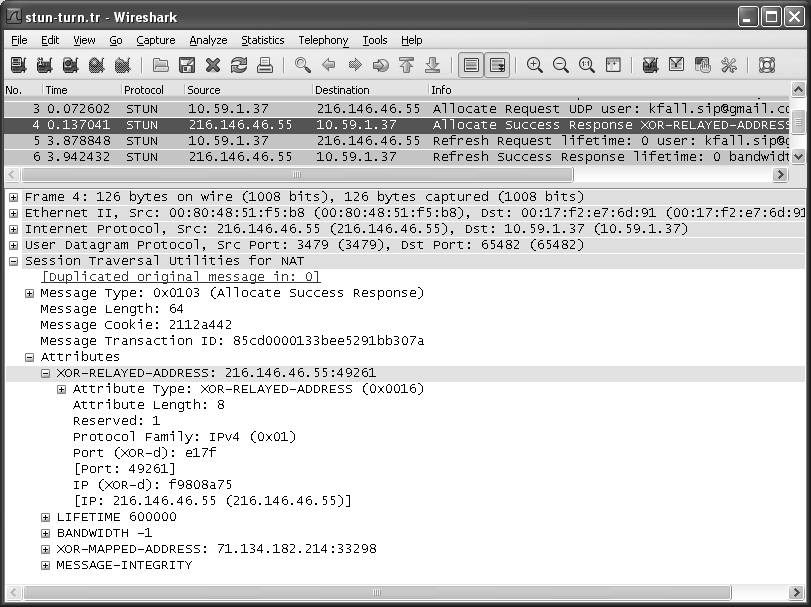
\includegraphics[scale=0.5]{imgs/7/7-15.png}
	\caption{一个 TURN 分配成功响应。报文是受到完整性保护的,包括了用于确定由 TURN服务器分配的端口和地址的XOR-RELAYED-ADDRESS 属性。如果不刷新的话,分配将被删除}
\end{figure}

正如前面提到的,TURN存在的缺点是流量必须通过TURN服务器进行中继,这可能
会导致低效的路由(即TURN服务器可能会离客户端和最优的对等客户端距离较远)。此外,
其他某些从对等到客户端的流量内容并不会通过TURN服务器。这包括ICMP值(见第8
章)、TTL(跳数限制)字段值和IP DS 字段(DS feld)值。此外,请求 TURN 的客户端必须
实现 STUN 长期信任机制,并有由TURN服务器操作员分配的登录凭证或账户。这有助于
避免不加控制地使用开放TURN 服务器,但也增加了配置的复杂度。

\subsection{交互连接建立}

鉴于 NAT的广泛部署及各种为穿越它们所必须采用的机制,一种称交互式连接建立
(Interactive Connectivity Establishment,ICE)\href{https://www.rfc-editor.org/rfc/rfc5245}{[RFC5245]}的通用功能被发展出来,用于帮助
位于NAT后的UDP 应用程序主机建立连接。ICE是一套启发式,利用它应用程序能够以
一个相对可预见的方式来执行 UNSAF。在它的操作中,ICE使用了其他协议,如TURN和
STUN。有一种方法可以扩展ICE 使其支持基于TCP 的应用[IDTI]。

ICE 使用并扩展了“请求/应答”协议,如单播SIP连接建立时的会话描述协议(SDP)
\href{https://www.rfc-editor.org/rfc/rfc3264}{[RFC3264]}。这些协议会提供一项拥有一组服务参数的服务,还包括一组选定的选项。找到
ICE 客户并纳入使用SDP/SIP 建立通信的VoIP 应用已经变得越来越普遍。然而在这种情况
下,ICE 被用于建立媒体流(如使用 RTP\href{https://www.rfc-editor.org/rfc/rfc3550}{[RFC3550]}或 SRTP\href{https://www.rfc-editor.org/rfc/rfc3711}{[RFC3711]}通话中的音频或视
频部分)的NAT 穿越,而另一种称为SIP 出站(SIP outbound)的机制\href{https://www.rfc-editor.org/rfc/rfc5626}{[RFC5626]}用于处理
SIP 信令,如谁是被叫方。尽管在实际中,ICE 主要用于基于 SIP/SDP 的应用,它也可以作
为一个通用的NAT 穿越机制用于其他应用程序。这样的一个例子就是将ICE定义为可扩展
的报文和现场协议(Extensible Messaging and Presence Protocol, XMPP) \href{https://www.rfc-editor.org/rfc/rfc6120}{[RFC6120]} 核心的
一个扩展,并与Jingle 一起使用[XEP-0176]。

通常,ICE用于创建两个 SDP实体(称代理(agent))的通信,首先需要确定一组
每个代理都能够用来与其他代理进行通信的候选传输地址(candidate transport address)。参
照图 7-11,这些地址可能是主机传输地址、服务器反向地址或中继地址。ICE 可同时使用
STUN 和TURN 来确定候选的传输地址。接着,ICE 根据优先分配算法对这些地址进行排序。
相比于那些需要中继的地址,该算法为能够提供直接连接的地址分配更大的优先级。然后,
ICE 为对等代理提供优先的地址集合,其中对等代理也会有类似的行。最终,两个代理商
量好一套最好的可用地址,并将选择的结果告知对方。使用一系列编码为STUN报文的检查
(check)可用于确定哪些候选的传输层地址是可用的。ICE 通过几项优化可以减少同意选定
候选地址的延迟,但这超出了本文的讨论范围。

ICE 开始试图发现所有可用的候选地址。这些地址可能是本地分配的传输层地址(如果
是多宿主代理便有多个主机)、服务器反向地址,或由TURN 确定的中继地址。在为每个地
址分配一个优先级后,每个代理使用SDP将优先级列表发送给对等方。对等代理执行相同
的操作,这导致每个代理会有两个优先名单。然后每个代理通过连接2个列表形成一个完全
相同的优先候选对(candidate pair) 集合。采用特定的顺序在候选对中执行一系列的检查可
以确定最终采用哪些地址。一般情况下,优先排序更加倾向于具有较少 NAT或者中继的候
选对。一个由ICE 指派的控制代理(controlling agent)将确定最终选择的候选对。控制代理
根据其优先顺序指定(nominate)使用哪个有效的候选对。控制代理可能会尝试所有对,并
随后做出选择(称常规选择(regular nomination)),或者可能使用第一个可行的对(称积
极选择 (aggressive nomination))。通过一个用于指定特定对的STUN 报文中的标志来表示常
规选择,而通过在每个请求中设置选择标志来表示积极选择。

利用被检查的地址信息在两个代理中交换 STUN 绑定请求信息,就是发送检查。检查是
由计时器触发,或者受来自于对等代理连接的调度(称触发检查(triggered check))。通过
包含地址信息的STUN绑定回复表示响应。在某些情况下这可能会揭示一个新的用于代理的
服务器反向地址(例如,当STUN 或者 TURN服务器最初确定候选地址后,代理之间又使用
了一个新的不同于以往的NAT)。如果发生这样的情况,代理获得了一个称为对等反向候选
(peer-refexive candidate)的新地址,该地址将被ICE 添加到候选地址中。ICE 检查是通过使
用基于 STUN 短期信任机制的完整性检查及 STUN 的 FINGERPRINT属性来完成的。当采
用TURN 时,ICE 客户机用TURN权限来限制针对感兴趣的远端候选地址的TURN 绑定。

ICE 采用了不同的实现概念。Lite 实现是专为没有采用 NAT 的系统部署所设计的。它们
永远不会充当控制代理,除非与另一个 Lite 实现进行交互。它们也不会执行前面提到的完全
(full)实现所做的检查。发出的STUN 报文会表明ICE实现的类型。所有ICE实现必须遵守
STUN\href{https://www.rfc-editor.org/rfc/rfc5389}{[RFC5389]},但 Lite 实现将永远只能充当STUN服务器。ICE通过表7-4中所述的属性
扩展 STUN。

名称

'PRIORITY

USE-CANDIDATE

表7-4 由ICE 定义的 STUN 属性

值

0x0024

0×0025

目的/ 用处

计算出相关候选地址的优先级

通过控制代理来指示选择候选地址

防火樯和网络地址转换

235

(续)

名称

ICE-CONTROLLED

ICE-CONTROLLING

值

0×8029

0x802A

目的丿用处

指示报文的发送者就是被控制的代理

指示报文的发送者就是控制代理

检查是一个包含PRIORITY属性的STUN绑定请求。该值等于由4.1.2节描述的算法
所指定的值\href{https://www.rfc-editor.org/rfc/rfc5245}{[RFC5245]}。当发送方是正在控制或者被控制的代理时,STUN 请求中会分别包
含 ICE-CONTROLLING 和 ICE-CONTROLLED 属性。一个控制代理可能还包括一个 USE-
CANDIDATE 属性。如果存在,这种属性指示控制代理在后续使用中想要选择的代理。

\section{配置包过滤防火墙和 NAT}

NAT 通常只需很少的配置(除非端口转发正在使用),但是防火墙通常需要进行配置,
有时它们需要大量的配置。大多数家庭网络中,同一台设备需要同时提供NAT、IP 路由和
防火墙等功能,并可能需要一些配置。虽然每个配置在逻辑上是独立的,但是配置文件、命
令行界面、网页控件或其他网络管理工具有时会合并。

\subsection{防火墙规则}

包过滤防火墙,必须给予一套说明匹配条件的指令来选择丢弃或者转发流量。现在配
置一个路由器,网络管理员通常配置一个或多个 ACL。每个 ACL 包含一个规则列表,其中
每个规则通常包含模式匹配条件(pattern-matching criteria)及其对应的动作(action)。匹配
条件通常允许规则表达网络层或传输层中的包字段值(例如,源和目的地IP 地址、端口号、
ICMP 类型字段等)以及方向(direction)的说明。方向模式采用基于方向的方式来匹配流量,
允许不同的规则集分别应用于传入与传出的流量。许多防火墙还允许在处理顺序中的某一点
应用防火墙规则。这方面的例子包括能够在IP 路由决策过程之前或之后指定一个ACL。在
某些情况下(尤其是当使用多个接口时),这种灵活性就变得很重要。

当一个包到达时,在适当的ACL 中按照顺序匹配其中的匹配条件。对于大多数的防火
墻而言,按照第一个匹配的规则采取动作。典型动作包括阻止或加速符合某项规则的流量,
还可以调整计数器或写一个日志条目。一些防火墙可能也包括附加功能,如将特定的数据包
发往应用程序或其他主机。每个防火墙厂商通常有自己的方法来指定规则,其中思科系统的
ACL 格式已成为许多企业级路由器厂商所广泛支持的一种格式。家庭用户的ACL 配置通常
使用一个简单的Web 界面。

一个非常流行的用于构建防火墙的系统是包含在现代版本 Linux 中的iptables,它是使
用一个称为 NetFilter[NFWEB] 的网络过滤功能来构建的。这是早先称为 ipchains 功能的演
变,iptables 能够提供无状态和有状态包过滤以及 NAT 和 NAPT 的支持。我们应研究它是如
何工作的,以更好地理解防火墙以及现代 NAT 提供的各种功能。

iptables 包含过滤表格(table)和过滤链(chain)的概念。一个表格包括许多预定义
的链,也可能包含0个或者多个用户自定义的链。三个预先定义的表格为:filter,nat 和
mangle。默认的 filter 表格用来处理基本的包过滤,包括了预先定义的 INPUT、FORWARD
和OUTPUT三条链。这些动作分别对应于目的地是防火墙路由器本身运行程序的流量、路
由时通过防火墙的流量以及从该防火墙主机发出的流量。nat 表格包含了 PREROUTING、
OUTPUT 和 POSTROUTING三条链。mangle 表格有五条链,主要用于任意修改数据包。

每条过滤链是一个规则列表,每条规则包含匹配条件及其对应的动作。这个动作(也
称为目标(target))可能是执行一条用户自定义的链或者执行如下预定义的动作:ACCEPT
DROP,QUEUE 和 RETURN。当一个数据包匹配上述之一的规则时,便立即采取响应的动
作。ACCEPT (DROP)是指数据包将被转发(丢弃)。QUEUE 是指数据包将被提交给一个用
户程序处理,RETURN 是指处理将在之前触发的一条链中继续,形成了一种包过滤链子调用。

一个完整的防火墙配置设计是非常复杂的,而且针对用户特定需求和它们所需要的服
务类型,因此我们不会在此尝试穷举每一个。相反,下面的例子只是给出了 iptables 中一小
部分可能的用法。下面的例子给出了一个 Linux 防火墙配置文件。它是由一个 shell触发的,
如 bash:

\begin{verbatim}
    
EXTIF="exto"

INTIF="etho"

LOOPBACK INTERFACE="10"

ALL="0.0.0.0/0"

# matches al1

# set default filter table policies to drop

iptables -P INPUT DROP

iptables -P OUTPUT DROP

iptables -P FORWARD DROP

# all local traffic OK

iptables -A INPUT -1 SLOOPBACK\_INTERFACE -j ACCEPT

iptables -A OUTPUT -i SLOOPBACK\_INTERFACE -j ACCEPT

# accept incoming DHCP requests on internal interface

iptables -A INPUT -i $INTIF -p udp -s 0.0.0.0\

--sport 67 -d 255.255.255.255 --dport 68 -j ACCEPT

# drop unusual/suspect rCP traffic with no flags set

iptables -A INPUT -P tcP --tcP-flags ALL NONE -j DROP
\end{verbatim}

这个例子说明了用户在设置一个过滤规则列表时的灵活性。初始时,所有的链都采用
默认规则(-P选项),将会影响所有没有匹配上规则的数据包。通过设置 filter 表中的 INPUT
和OUTPUT 链,所有进出本计算机(采用伪接口(pseudo interface)1o 表示)的流量都被设
置ACCEPT(即接受)。其中,j选项意味着“跳转”到一个特定的处理目标。接下来,
从IPv4地址0.0.0.0进来的UDP广播流量,以及目的地采用DHCP 端口号(67,68)的本
地/子网广播流量,都经由内部接口被允许通过。接着,将所有进来的TCP 段(参见第13
章)的标志(Flags)字段和1(ALL)相与(AND),再将结果与0(NONE)比较。当所有的
标志字段都为0时匹配成功,说明这不是一个非常有用的TCP段(正常情况下,第一个 TCP
段包含SYN标志位,其后的每个 TCP 段将包含一个有效的ACK 标志位)。

尽管这个例子所阐明的语法是针对 iptables 的,但是它的功能却不是。多数过滤性防火
墙都能够执行类似的检查和动作。

\subsection{NAT 规则}

在多数简单的路由器中,NAT能够配置为和防火墙一起工作。在基本的Windows 系统
中,NAT 被称互联网连接共享(Internet Connection Sharing,ICS),在 Linux 中被称为IP
伪装(IP masquerading)。以 Windows XP 为例,ICS有一些独有的特征。它为运行ICS 的主
机分配了 192.168.0.1 的“内部”IPv4地址,同时启动了一个 DHCP服务器和 DNS服务器。
其他的主机地址从 192.168.0/24子网段中分配,并将ICS主机作为DNS服务器。因此,在
已经有其他的主机或者路由器提供了上述服务或者存在地址冲突的网络中,ICS 不应该被启
用。通过修改注册配置能够修改默认的地址范围。

在 Windows XP 中为一个互联网连接启动ICS可以通过网络设置向导来完成,或者在一
个已经运行了的互联网连接中改变“高级”属性(在“配置|网络连接”中)。至此,用户可
能决定允许别的用户来控制或者关闭共享网络连接。这个功能也被称互联网网关设备发现
和控制(Internet Gateway Device Discovery and Control,IGDDC),它采用了通用的即插即用
的框架,允许在一个客户机中控制本地互联网网关,该内容在7.5.3 节中有介绍。所支持的
功能包括连接、断开,同时读取各种状态信息。与ICS一起工作的Windows 防火墙功能支
持创建服务定义(service definition)。服务定义等同于之前定义的端口转发。为了使之有效,
需要选中互联网连接中的“高级”属性标签,再添加一个新的服务(或者编辑一个现有的服
务)。然后,用户在外部接口和内部服务器中便能够填入合适的TCP 和UDP端口号。这样
也为进来的连接提供了一种配置 NAPT的方法。

和Windows一样,Linux 也将伪装功能和防火墙实现结合在一起。下面的脚本以一种简
单的方式来配置伪装。注意这种脚本是用来说明的,并不建议在产品中推荐使用。

\begin{verbatim}
    
EXTIF="ext0"

echo "Default FORWARD policy: DROP"

iptables -P

FORWARD DROP

echo

"Enabling NAT

on $EXTIF for hosts 192.168.0.0/24"

iptables -t nat -A POSTROUTING -O $EXTIF -s 192.168.0.0/24\

-j MASQUERADE

echo "FORWARD policy: DROP unknown traffic"

iptables

-A INPUT -i SEXTIF -m state

--state NEW, INVALID -j DROP

iptables -A FORWARD -i $EXTIF -m state --state NEW, INVALID -j DROP
\end{verbatim}

此处,filter 表格中FORWARDING链的默认策略被设置为DROP。在路由已经决定采
取哪个合适的外部接口时,下一个项目是对从192.168.0.0/24子网中获取了IPv4 地址的主机
流量的地址进行重写(通过NAT 中的nat表格和-t nat选项来实现)。由于NAT 的有状态的
工作方式,目前将有可能调整filter表格的规则以只允许为 NAT所知的连接的流量通过。最
后的两行调整了 INPUT和 FORWARD链,将丢弃任何无效或者未知(NEW)的传入流量。
特的操作符 NEW 和 INVALID 是在 iptables 命令之内定义的。

\subsection{与 NAT 和防火墙的直接交互:UPnP、NAT-PMP 和 PCP}

在多数情况下,一个客户系统希望或者需要和防火墙直接交互。例如,一个防火墙需要
为不同的服务配置或者再配置,以保证针对特定端口的网络流量不会被丢弃(创建一个“小
孔”)。在一个代理防火墙正在被使用的情况下,每个客户机必须被告知代理的身份。否则的
话,就无法越过防火墙进行通信。目前已经开发了许多支持客户机和防火墙之间进行通信的
协议。其中两个最为流行的是通用即插即用(Universal Plug and Play,UPnP)和 NAT端口
映射协议(NAT Port Mapping Protocol, NAT-PMP)。UPnP 这个标准是由一个称为 UPnP论
坛的工业组开发的。NAT-PMP 目前是IETF 中一个到期的草稿文件。NAT-PMP 为绝大多数
的Mac OS 系统所支持。UPnP 在 Windows 系统中是原生支持的,也能够被添加到 Mac OS
和 Linux 系统。UPnP 也被数字生活网络联盟(DLNA)[DLNA]用于家庭网络中支持消费电
子设备发现协议。

通过采用UPnP,被控制的设备通过第一个 DHCP来配置IP 地址,如果 DHCP 不可用
的话,就采用动态链接-本地地址配置(参见第6章)。接着,简单服务发现协议(Simple
Service Discovery Protocol, SSDP) [XIDS] 向控制点(例如,客户机)宣布设备的存在,
同时允许控制点来查询设备的其他信息。SSDP 使用了基于UDP 的两个 HTTP变种来代
替更为标准的TCP,它们被称为HTTPU 和 HTTPMU[XIDMU],其中后者使用组播寻址
(IPv4 地址239.255.255.250,端口 1900)。如果使用基于IPv6的SSDP,那么将采用如下
的地址:ffO1:C(本地节点),ff02:(本地连接),ff05:c(本地站点),ff08:c(本地组织),
ffOe::c(全局)。

后续的控制和事件通知(eventing)是由通用事件通知架构(General Event Notification
Architecture,GENA)控制的,它采用了简单对象访问协议(Simple Object Access Protocol,
SOAP)。SOAP支持客户/服务器远程过程调用(Remote Procedure Call,RPC)机制,使
用编码在可扩展标记语言(eXtensible Markup Language,XML)中的报文(XML 通常用于
Web 网页中)。UPnP 被消费电子设备所广泛采用,包含音频和视频回放和存储设备。NAT
和防火墙设备是采用互联网网关设备(Internet Gateway Device,IGD)协议控制的[IGD]。
IGD 支持一些别的功能,包括学习 NAT 映射和配置端口转发的能力。感兴趣的读者可以从
MiniUPnP 项目主页[UPNPC]中得到一个简单的IGD 客户端用于实验。UPnP IGD 的第二个
版本[IGD2]增加了对IPv6的支持。

UPnP是一个包含 NAT 控制及其他不相关规范的广泛架构,而NAT-PMP 是另外一种方
法,它针对与NAT设备进行程序通信。NAT-PMP 是苹果公司用于零配置网络的服务器搜索
协议 Bonjour 规范的一部分。NAT-PMP 并没有采用发现过程,这是由于被管理的设备通常
就是可通过DHCP获取的默认网关。NAT-PMP 使用UDP端口 5351。NAT-PMP 支持一个用
于学习 NAT外部地址和配置端口映射的请求/响应协议。它也支持一个基本的事件机制,当
NAT外部地址发生改变时能够通知监听者。这是在外部地址发生改变时通过采用一个 UDP
组播报文发送到地址 224.0.0.1(即所有主机的地址)来完成的。NAT-PMP 使用UDP端口号
5350用于客户机/服务器的交互,5351端口用于组播事件通知。根据端口控制协议(Port
Control Protocol, PCP) [IDPCP]的建议,NAT-PMP 的概念可被扩展用于支持 SPNAT。

\section{IPv4/IPV6 共存和过渡中的 NAT}

随着最后一个顶层单播IPv4地址在2011年早期被分配出去,向IPv6的过渡便开
始加速了。曾经认为通过为主机配备双栈功能(例如,实现完整的IPv4 和 IPv6协议栈)
\href{https://www.rfc-editor.org/rfc/rfc4213}{[RFC4213]},网络服务就会过渡到只有IPv6 的操作。目前认为IPv4 和 IPv6将会共存更长一
段时间,甚至可能是无限期的,这是由于各种经济原因网络基础设施可能会使用IPv4 或者
IPv6或者两者同时使用。假设这是真的,那就需要支持IPv4 和 IPv6系统之间的通信,无论
它们是否拥有双协议栈。目前用于支持IPv4和IPv6组合的两种主要方法是隧道和转换。隧
道方法包括Teredo(见第10章)、双协议栈精简版(DS-Lite)和 IPv6快速部署(6rd)。虽然
DS-Lite 采用SPNAT作为其架构的一部分,但在\href{https://www.rfc-editor.org/rfc/rfc6144}{[RFC6144]}描述的框架中给出了一种更单一
的转换方法,它使用了我们在第2章中见到过的嵌入了IPv4的IPv6地址。我们将在本节了
为详尽地讨论 DS-Lite 和转换架构的细节。

\subsection{双协议栈精简版}

DS-Lite(Dual Stack Lite,双协议栈精简版)\href{https://www.rfc-editor.org/rfc/rfc6333}{[RFC6333]}是一种希望在内部运行IPv6的
服务提供者更容易过渡到IPv6(同时支持传统的IPv4用户)的方法。从本质上讲,它可以
让供应商把重点放在部署一个可操作的IPv6核心网上,还通过使用少数的IPv4地址为客
户提供了IPv4 和IPv6连接。该方法结合了在IPv6 中的IPv4 (IPv4-in-IPv6)的“软电线”
(softwire) 隧道与 SPNAT\href{https://www.rfc-editor.org/rfc/rfc5571}{[RFC5571]}。图7-16显示了这种部署的设想。

图7-16
DS-Lite 通过使用一个只有IPv6的架构使服务提供者能够支持IPv4和IPv6 客户网络。通过
在服务提供者边缘使用 SPNAT,能够最大限度地减少IPv4 的使用

在图7-16中,每个客户网络运行IPv4 和IPv6的任意组合。假定仅使用IPv6 来管理服
务提供者的网络。客户对IPv6互联网的访问是通过采用传统的IPv6路由来完成的。对于
IPv4 的访问,每个客户使用一个特殊的“前”网关(在图7-16中标记为“B4”)。一个B4
设备提供了基本的IPv4服务(如DHCP服务,DNS代理等),但也以多点到点的隧道方式封
装了客户的IPv4流量,并在“后”设备(图7-16中标记为“AFTR”)处终止。这个 AFTR
设备为目标是IPv4互联网的流量执行了解封操作,并为相反方向的流量执行封装操作。
AFTR还执行了 NAT,并作为一种形式的SPNAT。更具体地说,AFTR 可以利用客户隧道终
端的标志信息来消除从 IPv4 互联网返回到 AFTR的流量的二义性。这将允许多个客户使用
相同的IPv4地址空间。通过利用 DHCPv6中的一个 AFTR-Name 选项\href{https://www.rfc-editor.org/rfc/rfc6334}{[RFC6334]},一个 B4
设备能够学习到它所对应的 AFTR设备的名称。

回忆一下第6章中对IPv6快速部署(6rd)的讨论是非常有益的。鉴于 DS-Lite 通过一
个服务提供者的IPv6网络为客户提供了到IPv4 的访问,6rd 的目标是通过一个服务提供者
的IPv4 网络为客户提供到 IPv6的访问。本质上,它们使用类似的框架组件,但却来取了相
反的做法。然而,6rd 中从IPv6地址映射到相应的IPv4 隧道端点(反之亦然)的计算,是通
过一个无状态的地址映射算法完成的。框架中也使用了无状态地址转换,用于IPv4 和 IPV6
之间的全协议转换,这是我们接下来需要讨论的。

\subsection{使用 NAT 和 ALG 的 IPv4/IPV6 转换}

采用隧道技术解决IPv4 和IPv6共存问题的最大缺点是,采用一种地址类型的主机上
的网络服务无法被采用了另一种地址类型的主机直接访问。由此,一个只有IPv6 的主机就
只能够与其他支持 IPv6 的系统进行通信。这种状况是不能接受的,因为只支持IPv6 的新系
统将无法访问在传统的IPv4互联网上提供的服务。为了解决这个问题,在2008年至2010
年间花了很大的努力开发了一个能够直接在IPv4 和IPv6间进行转换的框架。借鉴 NAT-
PT\href{https://www.rfc-editor.org/rfc/rfc2766}{[RFC2766]}已有的糟糕经验,这个框架被认为太脆弱了,针对今后不断变化的使用也没有
可扩展性,因此最终被舍弃了\href{https://www.rfc-editor.org/rfc/rfc4966}{[RFC4966]}。

IPv4 和IPv6转换的框架在\href{https://www.rfc-editor.org/rfc/rfc6144}{[RFC6144]}中有描述。这个基本的转换架构同时采用了有状
态的和无状态的方法来完成IPv4 和IPv6地址之间的转换、DNS 的转换(参见第11章),以
及在任何必要情况下(包括ICMP 和FTP)添加的行或者ALG 的定义。本节我们将讨论的
内容包括基于\href{https://www.rfc-editor.org/rfc/rfc6145}{[RFC6145]}和\href{https://www.rfc-editor.org/rfc/rfc6146}{[RFC6146]}的有状态和无状态的IP地址转换,以及第2章中讨
论过的源于\href{https://www.rfc-editor.org/rfc/rfc6052}{[RFC6052]}的寻址。其他针对特定协议的转换问题将在后续的章节中讨论。

\subsubsection{已转换的IPv4 地址和可转换的IPv4地址}

在第2章,我们已经讨论了内嵌有IPv4的IPv6地址结构。这样的地址是IPV6地
址,但是将其作为一个函数的输入,则能够输出一个对应的IPv4地址。这个函数也能轻
易地被反转。内嵌IPv4的IPv6地址存在两种重要的类型,称已转换的IPv4地址(IPv4-
converted address) 和可转换的IPv4地址(IPv4-translatable address)。每个提到的地址类型
是其他类型的一个子集。也就是说,如果我们将每个地址类型看作一个集合,那么会有(可
转换的IPv4)C(已转换的IPv4)C(内嵌的IPv4)C(IPv6)。可转换的IPv4地址是能够
通过有状态的方式来确定一个 IPv4 地址的IPv6地址(参见7.6.2.2节)。

IPv4 和IPv6地址之间的算法转换涉及使用第2章中讨论过的前缀。这个前缀可能是
一个知名前缀(WKP) 64:ff9b::/96 或者另外一个为服务提供者所有并和转换器一起使用的
特定于网络的前缀。WKP 只用于表示常规的全局可路由的IPv4地址,不能表示私有地址
\href{https://www.rfc-editor.org/rfc/rfc1918}{[RFC1918]}。此外,WKP也不能用于创建可转换的IPv4地址。这样的地址应该在服务提供
者网络内部被定义,因此不适合在一个全局范围中使用。

WKP 是很有趣的,因为相对于 Internet 校验和,它是校验和中立(checksum-neutral)
的。回想一下第5章介绍的 Internet 校验和的计算方法。假如我们将前缀64:ff9b::/96看作
是十六进制值0064,ff9b,0000,0000,0000,0000, 0000,0000组成的,这些值的和是 ffff,它
的补码正好是0。因此,当一个 IPv4 地址包含 WKP 前缀时,包中作为转换结果(例如,在
IPV4 头部中的 TCP或者 UDP 校验和)的相关 Internet 校验和是不会受影响的。自然地,恰
当选择的特定于网络的前缀也能是校验和中立的。

在接下来的两个小节中,我们将使用符号To4(A6,P)来表示从前缀为P的IPv6地
址A中得到的IPv4地址。P可以是WKP 或者是某个特定于网络的前缀。我们将使用符号
To6(A4,P)来表示从前缀为P的IPv4地址A中得到的IPv6地址。注意,除了一些特殊的
情况之外,A6 = To6(To4(A6,P),P) 和 A4 = To4(To6(A4,P),P)。

\subsubsection{无状态转换}

无状态的 IP/ICMP 转换(Stateless IP/ICMP Translation,SIIT)是指不采用状态表格进行
IPv4 和IPv6数据包转换的方法\href{https://www.rfc-editor.org/rfc/rfc6145}{[RFC6145]}。转换中无须查找表格,只需要使用一个可转换
的IPv4地址及一个预定义的用于转换IP头部的计划。大部分情况下,IPv4选项是不需要转
换的(被忽略),IPv6扩展头部也不需要转换(分片头部例外)。唯一的例外是未到期的IPv4
源路由选项。如果存在这种选项,数据包将被丢弃,并产生相应的ICMP 差错报文(目的不
可达,源路由失败,见第8章)。表7-5描述了当转换一个 IPv4报文到IPv6 时,IPv6 头部
字段是如何赋值的。

IPv6 字段

表7-5 当从IPv4转换到IPv6 时创建一个IPv6 头部的方法

分配方法

版本(Version)

DS 字段 /ECN (DS Field/ECN)

流标志(Flow Label)

负載长度(Payload Length)

下一个头部 (Next Header)

跳数限制 (Hop Limit)

源 IP 地址 (Source IP Address)

目的IP 地址(Destination IP Address)

设置 6

拷贝自 IPv4 头部中的相同值

设置为0

设置为IPv4 的总长度减去 IPv4 头部长度(包含选项)

设置IPv4 协议字段(或者58,如果协议字段值为1)

设置为44来表示是一个分片头部,如果创建的IPv6 数据报是一个

分片或者 DF位没有被设置

设置为IPv4 TTL 字段减去1(如果这个值为0,则该报文将被丢弃,

同时产生一个ICMP超时报文,参见第8章)

设置6(IPV4源IP 地址,P)

设置次6(IPv4 目的IP地址,P)

在转换的过程中,IPv4 头部被抽离,取而代之的是IPv6头部。假如到达的IPv4 数据报
相对于下一个链路的 MTU来说太大了,并且其头部中的DF 位也未设置,那么将会产生多
个IPv6 分片数据包,其中每个将包含一个分片头部。当到达的IPv4数据报是一个分片时,
也会发生这种情况。\href{https://www.rfc-editor.org/rfc/rfc6145}{[RFC6145]}建议当到达的IPv4数据报头部的DF 位值0时,不管转换
器是否需要执行分片,也不管达到的数据报是否是一个分片,都需要在结果 IPv6 数据报中
包含一个分片头部。这将允许IPv6接收者知道IPv4的发送者并没有采用PMTUD。当包含
了一个分片头部时,需要根据表7-6所列的方法来设置字段值。

分片头部字段

下一个头部 (Next Header)

分片偏移(Fragment Offset)

更多分片位(More Fragments Bit)

标识(Identification)

表7-6从IPv4 到IPV6转换时为分片头部中字段赋值的方法

分配方法

设置为IPv4中的协议字段

拷贝自 IPv4 分片偏移字段

拷贝自 IPv4 中的更多分片(M) 位字段

低16位根据IPv4 中的标识字段设置。高16位设置为0

在相反的方向(IPv6到IPv4转换)上会涉及创建一个 IPv4数据报,并根据到达的IPv6
头部字段值来设置该头部字段值。显然,范围更广的IPv6地址空间不可能允许一个只有
IPV4 的主机访问IPv6互联网上的每一台主机。当一个未分片的IPv6 数据报到达时,表7-7
给出的方法能给传出的IPv4 数据报头部的字段赋值。

表7-7 将一个未分片的IPv6 数据报转换为IPv4 时用于创建IPV4 头部的方法

IPv4 头部字段

分配方法

版本(Version)

IHL

DS 字段/ECN (DS Field/ECN)

总长度(Total Length)

标识(Identification)

标志 (Flags)

分片偏移(Fragment Offset)

TTL

设置为4

设置5(没有IPv4选项)

拷贝自 IPv6 头部中的相同值

IPv6 中负载长度字段值加上20

设置为0(可以选择设置为其他一些预设的值)

更多分片(M)设置0;不分片(Don't Fragment)(DF)设置1

设置力0

IPv6 中跳数限制字段值减去1

(续)

IPV4 头部字段

协议(Protocol)

头部校验和(Header Checksum)

源IP地址 (Source IP Address)

目的IP 地址 (Destination IP Address)

分配方法

拷贝自 IPv6 的第一个下一个头部字段,不涉及分片头部、HOPOPT、

IPv6-Route 或者 IPv6-Opts。将值58改变1来支持ICMP(参见第8章)

为新创建的IPv4头部而计算

To4(IPV6源IP地址,P)

To4(IPv6目的IP 地址,P)

假如到达的一个 IPv6 数据报包含一个分片头部,将采用从表7-7修改而来的赋值方法
来为传出的IPv4数据报字段赋值。表7-8给出了这种情况。

表7-8

IPv4 头部字段

总长度(Total Length)

标识(Identification)

当转换一个分片的IPv6 到IPv4时用于创建IPv4头部的方法

标志(Flags)

分片偏移(Fragment Offset)

分配方法

IPv6 负载长度字段值減去8加上20

拷贝自 IPv6 分片头部标识字段中的低16位

更多分片(M)拷贝自IPv6分片头部中的M位字段。不分片(DF)设

置为0以便允许 IPv4 网络中的分片

拷贝自IPv6分片头部中的分片偏移字段

在分片 IPv6数据报的情况下,转换器将生成分片的IPv4报文。注意在IPV6中标识
(Identification)字段更大,假如来自于同一台主机的多个不同的IPv6数据报被分片了,并且
它们的标识字段共享了一个低16位值,这些分片将可能无法重组。但是,这种情况的危险
性低于传统的IPv4的标识字段中出现的环绕情况。况且,更高层次上的完整性检查将大大
打消这种顾虑。

\subsubsection{有状态的转换}

在有状态的转换中,NAT64\href{https://www.rfc-editor.org/rfc/rfc6146}{[RFC6146]}被用于支持只有IPv6的客户机与其他IPv4服
务器进行通信。当许多重要的服务继续只用IPv4来提供时,这将显得非常重要。针对头部
的转换方法与7.6.2.2节中介绍的无状态转换方法几乎一样。作为一个 NAT,NAT64符合
BEHAVE 规格,支持独立于端点的映射,以及独立于端点和依赖于地址的过滤。因此,它是
和我们前面讨论过的 NAT穿越技术(如ICE、STUN、TURN)兼容的。缺乏这些附加协议,
NAT64仅支持由IPv6 主机发起的与IPv4 主机通信的动态转换。

NAT64 在跨越多个地址类型时像传统的NAT (NAPT)那样工作,除了从 IPv4到 IPv6
这个方向的转换比相反方向的转换更加简单。一个NAT64设备被赋予一个 IPv6 前缀,能用
于形成一个有效的IPv6地址,该地址是通过第2章和\href{https://www.rfc-editor.org/rfc/rfc6052}{[RFC6052]}描述的机制从 IPv4上直接
转换过来的。由于IPv4地址空间的不足,在IPv6到IPv4这个方向的转换利用了一个动态管
理的IPv4地址池。这需要 NAT64 支持NAPT的功能,据此多个不同的IPv6 地址可能会映
射到一个相同的IPv4地址上。NAT64目前定义了由IPv6 节点初始化的TCP、UDP 和 ICMP
报文的转换方法。(在ICMP 查询和应答的情况下,ICMP 标识符字段被用来代替传输层的端
口号,见第8章。)

NAT64处理分片不同于其有状态部分。对于到达的传输层校验和不为0的TCP或者
UDP 分片(见第10章),NAT64可能会将分片排队,然后一起或者单独地转换它们。NAT64
必须处理分片,即便是那些乱序到达的。一个 NAT64可能被配置一个时限,限制分片被缓
存的时间(至少2s)。否则,NAT 可能受到DoS攻击,耗尽保存分片的包缓冲空间。

\section{与防火墙和 NAT 相关的攻击}

鉴于部署防火墙的主要目的是减少攻击的风险,因此防火墙的缺点比终端主机或路由器
少一些也不奇怪。这就是说,它们不是没有缺点的。最常见的防火墙问题是由不完整或不正
确配置导致的。配置防火墙不是一个简单的任务,尤其是大型企业,其中许多服务需要每天
使用。其他形式的攻击利用了某些防火墙的弱点,包括其中许多防火墙(尤其是比较老的)
没有能力来处理IP分片。

一种类型的问题出现在 NAT/防火墙受到外部劫持,进而为攻击者提供伪装能力。如果
防火墙的配置启用了 NAT,那么在其外部接口到达的流量会被重写,因此这些流量看起来好
像是来自于NAT设备的,从而隐藏了攻击者的实际地址。更糟糕的是,从NAT 的角度来看
这是“正常”的行为,但它恰恰是从外面得到的输人数据包而不是在内部得到的。这是一个
在Linux 上基于ipchains 的NAT/防火墙规则的特定问题。最简单的设置伪装的配置
将会允许这种攻击发生,因此并不推荐。正如所看到的,它将默认策略设置为 MASQUERADE,
潜在地对任何IP实行转发。

\begin{verbatim}    
Linux# ipchains -P FORWARD MASOUERADE
\end{verbatim}


另一种与防火墙和 NAT规则相关的问题是,它们可能过时了。尤其是,它们可能包
含端口转发条目或其他所谓的小孔,允许已不存在的服务的流量通过。一个相关的问题是,
一些路由器将多个防火墙规则副本保存在内存中,路由器必须明确指示使用哪个规则。最
后,另一个常见的配置问题是当添加新的规则时,许多路由器将新、旧防火墙规则一起合并
(merge)了。如果操作者不知道这种行为的话,这将导致意想不到的结果。

与分片有关的问题是如何构造IP 分片。当一个 IP 数据报被分片时(见第10章),包含
了端口号的传输层头部只出现在第一个分片中,在别的分片中没有。这是分层和封装的TCP
IP 协议体系结构直接导致的结果。不幸的是对于防火墙而言,如果收到的分片不是一个的
话,它所提供的关于与该数据包相关联的传输层或者服务信息将会非常少。唯一明显的解决
方法是找到第一个分片(如果有的话),这显然需要一个有状态的防火墙,为此可能会遭到资
源耗尽攻击。即使是状态防火墙也可能功亏一篑:如果第一个分片在后续分片之后达到,防
火墙可能无法在过滤操作之前执行分片重组。在某些情况下,防火墙丢弃不能完全识别的分
片,这可能会给突然使用了大数据报的流量造成麻烦。

\section{总结}

防火墙为网络管理员提供了一种机制,限制那些可能对终端系统有害的信息流动。主
要有两种类型的防火墙:包过滤防火墙和代理防火墙。包过滤防火墙可进一步划分为有状态
的和无状态的,它们通常作为IP 路由器。有状态的防火墙更加复杂,能够支持更广泛的应
用层协议(在一个数据包流中能够横跨多个数据包执行更为复杂的登录和过滤操作)。代理
防火墙通常作为一种形式的应用层网关。对于这些防火墙,每个应用层服务在防火墙上必须
有自己的代理处理程序,这些处理程序可以修改通过的流量,甚至是其中的数据部分。如
SOCKS这类协议以标准化的方式支持代理防火墙。

NAT是一种机制,使得大量的终端主机可以共享一个或多个全局路由的IP地址。NAT
被广泛应用于上述目的,但也可以和防火墙规则结合形成一个 NAT/防火墙组合。在这种流
行的配置中,位于 NAT “背后”的主机允许发送流量到全球互联网,但是仅允许针对传出流
量的响应流量通过NAT返回。这为位于 NAT“背后”采用端口转发处理的服务提出了一个
小问题,如何允许目的地是 NAT 内开启了服务的主机的传入流量通过。通过在两个地址空
间之间转换地址,NAT 也被提出用于协助从 IPv4过渡到IPv6。此外,NAT 也正被考虑用于
ISP 内部,以进一步减轻IPv4地址耗尽的压力。如果这个大规模地发生,普通用户想在他们
的家庭网络中为 Internet 提供服务将变得更为困难。

一些应用程序使用了一套启发式,用于确定在 NAT后面的它们对外所采用的地址。其
中许多是单方面操作的,没有NAT 的直接帮助。这样的应用程序被认为使用了 UNSAF方
法,未必完全可靠。一组文件(由IETF 的BEHAVE工作组制定)指定了针对不同协议的
NAT正当行为,但并非所有的 NAT都实现这些规范。因此,可能需要采用NAT 穿越技术,
以确保连接可用。

NAT 穿越涉及确定一套可用于支持通信的地址和端口号集合,即使必须使用一个或多
个 NAT。STUN 是确定地址的主力协议。TURN 是一个特定的STUN 用法,通过一个通常位
于互联网的经过特配置的TURN服务器来中继流量。通过使用一整套 NAT 穿越协议,如
ICE,可以确定使用了哪些地址或者中继。ICE 通过使用本地信息和由 STUN 和 TURN确定
的地址来确定一对通信端点之间所有可能的地址。然后为后续的通信选择“最好”的地址。
ICE 机制已受到 VOIP 服务的广泛关注,后者采用SIP 协议发送信令。

防火墙和 NAT 可能需要配置。基本设置足够许多家庭用户使用,但是为了允许某些服
务能够正常工作,可能需要修改防火墙。此外,如果在 NAT后面的用户希望提供互联网服
务,就需要在 NAT 设备上配置端口转发。有些应用程序通过采用 UPnP 和 NAT-PMP 协议与
NAT设备直接通信来支持配置。当被支持和启用时,这将允许应用程序自动配置一个 NAT
端口转发和数据绑定,而无须用户干预。对于家庭用户在动态配置的 NAT(即面向 Internet
的IP 地址可能会变化)后运行一个 Web 服务器时,如动态 DNS(见第11章)之类的附加服
务,这也可能是很重要的。

\section{参考文献}

[ANM09] S. Alcock, R. Nelson, and D. Miles, 'Investigating the Impact of Service
Provider NAT on Residential Broadband Users/" University of Waikato, unpub-
lished technical report, 2009.

[DLNA] http://www.dlna.org

[HBA09] D. Hayes, J. But, and G. Armitage, "Issues with Network Address Trans-

lation for SCTP" Computer Communications Review, Jan. 2009.

[IDPCP] D. Wing, ed., S. Cheshire, M. Boucadair, R. Penno, and P. Selkirk, "Port

Control Protocol (PCP)." Internet draft-ietf-pcp-base, work in progress, July 2011.

[IDSNAT] R. Stewart, M. Tuexen, and I. Ruengeler, “Stream Control Transmission

Protocol (SCTP) Network Address Translation" Internet draft-ietf-behave-

sctpnat, work in progress, June 2011.

[DTI J. Rosenberg, A. Keranen, B. Lowekamp, and A. Roach, "TCP Candidates

with Interactive Connectivity Establishment (ICE)" Internet draft-ietf-mmusic-

ice-tcp, work in progress, Sep. 2011.

[IGDJ UPnP Forum, "Internet Gateway Devices (IGD) Standardized Device

Control Protocol V 1.0" Nov. 2001.

[IGD2] UPnP Forum, "TDG:2 Improvements over IGD:1,"'Mar. 2009.

[ISP] http://www.iana.org/assignments/stun-parameters

[MBCB08] O. Maennel, R. Bush, L. Cittadini, and S. Bellovin, "'A Better Approack
to Carrier-Grade-NAT"' Columbia University Technical Report CUCS-041-08,

Sept. 2008.

[NFWEBJ http://netfilter.org

[PJSUA] http://www.pjsip.org/pjsua.htm

[UPNP] http://www.upnp.org

[UPNPC] http://miniupnp.free.fr

[XEP-0176] J. Beda, S. Ludwig, P. Saint-Andre, J. Hildebrand, S. Egan, and R.

McQueen,“XEP-0176: Jingle ICE-UDP Transport Method,' XMPP Standards

Foundation, June 2009, http://xmpp.org/extensions/xep-0176.html

[XIDADJ P. Gauthier, J. Cohen, M. Dunsmuir, and C. Perkins, "Web Proxy

Auto-Discovery Protocol” Internet draft-ietf-wrec-wpad-01, work in progress

(expired), June 1999.

IXIDMU] Y. Goland, “Multicast and Unicast UDP HTTP Messages/" Internet

draft-goland-http-udp-01.txt,work in progress (expired), Nov. 1999.

IXIDPMP] S. Cheshire, M. Krochmal, and K. Sekar, "NAT Port Mapping Protocol

(NAT-PMP)." Internet draft-cheshire-nat-pmp-03.txt, work in progress (expired),

Apr.2008.

[XIDS] Y. Goland, T. Cai, P. Leach, Y. Gu, and S. Albright, "Simple Service Discov-

ery Protocol/1.0 Operating without an Arbiter/” Internet draft-cai-ssdp-V1-03.txt,

work in progress (expired), Oct. 1999.

348

B52